\documentclass{midl}
\usepackage{mwe}
\usepackage[english]{babel}
\usepackage{caption}
\usepackage{float}

\title[DLMI]{Lymphocytosis Classification Challenge}

\midlauthor{\Name{Joachim COLLIN} \Email{joachim.collin@eleves.enpc.fr}
\AND
\Name{Bastien LE CHENADEC} \Email{bastien.le-chenadec@eleves.enpc.fr}
\AND
\Name{Team: Lymphatigués}
}
\begin{document}

\maketitle

\begin{abstract}
    This report presents our approach to the Lymphocytosis Classification Challenge for the Deep Learning for Medical Imaging (DLMI) course. We first establish a simple baseline model using a convolutional neural network (CNN) on single images combined with patients attributes. We then explore two promising approaches that yield better results: an unsupervised classification model based on SCAN, and a mixture of experts model. We present the results of these models and discuss their performance.
\end{abstract}

\section{Introduction}
\label{sec:introduction}
Lymphocytosis is a common hematologic abnormality characterized by an increase in the absolute concentration of lymphocytes to more than 4000 lymphocytes/mL for adult patients \cite{Hamad_2023}. This condition can arise from various sources, including reactions to infections, drugs, or stress, or it may indicate a lymphoproliferative disorder, which is a type of cancer involving abnormal proliferation of lymphocytes. Clinicians typically diagnose lymphocytosis by assessing personal data such as medical history, symptoms, medication lists, and through a blood test to measure lymphocyte levels. However, additional tests may be necessary to confirm the cause of lymphocytosis and determine an appropriate treatment plan. Malignant lymphocytosis is a type of cancer, that should be treated as soon as possible to reduce and prevent further complications. While the diagnosis process is efficient, it suffers from poor reproducibility, and the additional tests required can be costly and time-consuming \cite{Sahasrabudhe_2021}. Being able to distinguish more accurately reactive from malignant lymphocytosis is a binary classification problem that could lead to a better identification of patients requiring additional testing. In this challenge, we aim to predict the malignancy of lymphocytosis using multiple blood smears for each patient, and their clinical attributes.

\subsection{Related work}

Radiomics used to rely on feature extraction to identify imaging attributes, and then, on feature selection to condense these attributes into a robust set, avoiding overfitting \cite{Vial_2018}. Nowadays, Deep Learning methods are able to learn from scratch more powerful deep representations \cite{Yao_2020}, making them the new standard. To adress weakly supervised learning problems, such as this challenge, MIL methods are usually adopted. In \cite{Sahasrabudhe_2021}, the authors tackle this very problem leveraging a multi-instance deep convolutional neural network, where the embeddings from each patient's images are aggregated before being associated with the patient's clinical attributes to make a prediction.


\section{Architecture and methodological components}
\label{sec:methodology}

The variable number of images per patient can be seen through two different perspectives: either as a multi-instance learning problem, where the model has to make a prediction based on a set of images, or as a weakly supervised learning problem, where there are missing labels for the images. These perspectives motivate different kind of architectures.

\subsection{Baseline}

Our baseline model is a simple convolutional neural network (CNN) with two convolutional layers followed by three fully connected layers. The annotations are concatenated with the flattened output of the last convolutional layer. This model predicts individual labels for each image, and the final prediction is the average of the individual predictions. While simple and fast to train, this model quickly gives good results on the test set.

Building on this baseline, we tried to improve the model by using a more complex architecture (VGG 16, VGG 19, U-Net, ResNet) and attention mechanisms, without much success. The limitation of these models is that they do not take into account the set of images as a whole. From a medical perspective, an individual image does not contain enough information to make a diagnosis, and the variety of images per patient is a source of information that has to be exploited.

\subsection{Unsupervised classification}

Encouraged by our intuition on the diversity of the images, we decided to try an unsupervised classification approach. If we can split the images in relevant classes, we can then use a simple machine learning model to predict the malignant nature of the lymphocytosis. We used the state-of-the-art unsupervised classification model SCAN \cite{van-gansbeke-2020}, which is based on a ResNet model\footnote{We did not include this code because we did not use this model in the end and the code for SCAN is huge.}. After training the model on our data with 20 class, we computed class confusions based on first and second ranked classes for each image. We then used these confusions to fuse the most similar classes and were left with 15 meaningful classes (figure \ref{fig:unsupervised_classification}). While these classes are not perfect, we hope that they can provide a good enough representation of the data to be used in a simple machine learning model. We compute the following features for each patient:

\begin{itemize}
    \setlength\itemsep{0em}
    \item Gender, lymphocyte count, age (3 features)
    \item Class proportions (15 features)
    \item Entropy of the class distribution (1 feature)
    \item Variety of classes (i.e. number of different image classes for the patient) (1 feature)
    \item Outliers: number of the above features that are greater in value than 90\% of the training samples (1 feature)
\end{itemize}

We run a 5-fold cross-validation with stratified splits and report the balanced accuracy of different machine learning models in figure \ref{fig:unsupervised_classification_models}. There is a lot of variability in the performance of the models, and only one model (GaussianNB) performs better than the baseline on every split. We thus chose to submit a prediction with this model, which did not beat the baseline on the test set. These results are disappointing, probably because the learned classes are not meaningful enough and a supervised approach would be more appropriate.

\subsection{Mixture of experts}
The poor results of the unsupervised classification approach led us back to a deep learning model, but this time we wanted to take into account the set of images as a whole. A natural way to do this is to compute a feature vector for each image, and then to aggregate these feature vectors for instance with mean pooling. We first tried this approach with a model similar to the baseline, but this did not yield good results and the training was very unstable. After some research, we decided to try an architecture inspired by \cite{Sahasrabudhe_2021}, which is detailed in figure \ref{fig:mixture_of_experts}.

\begin{figure}[H]
    \centering
    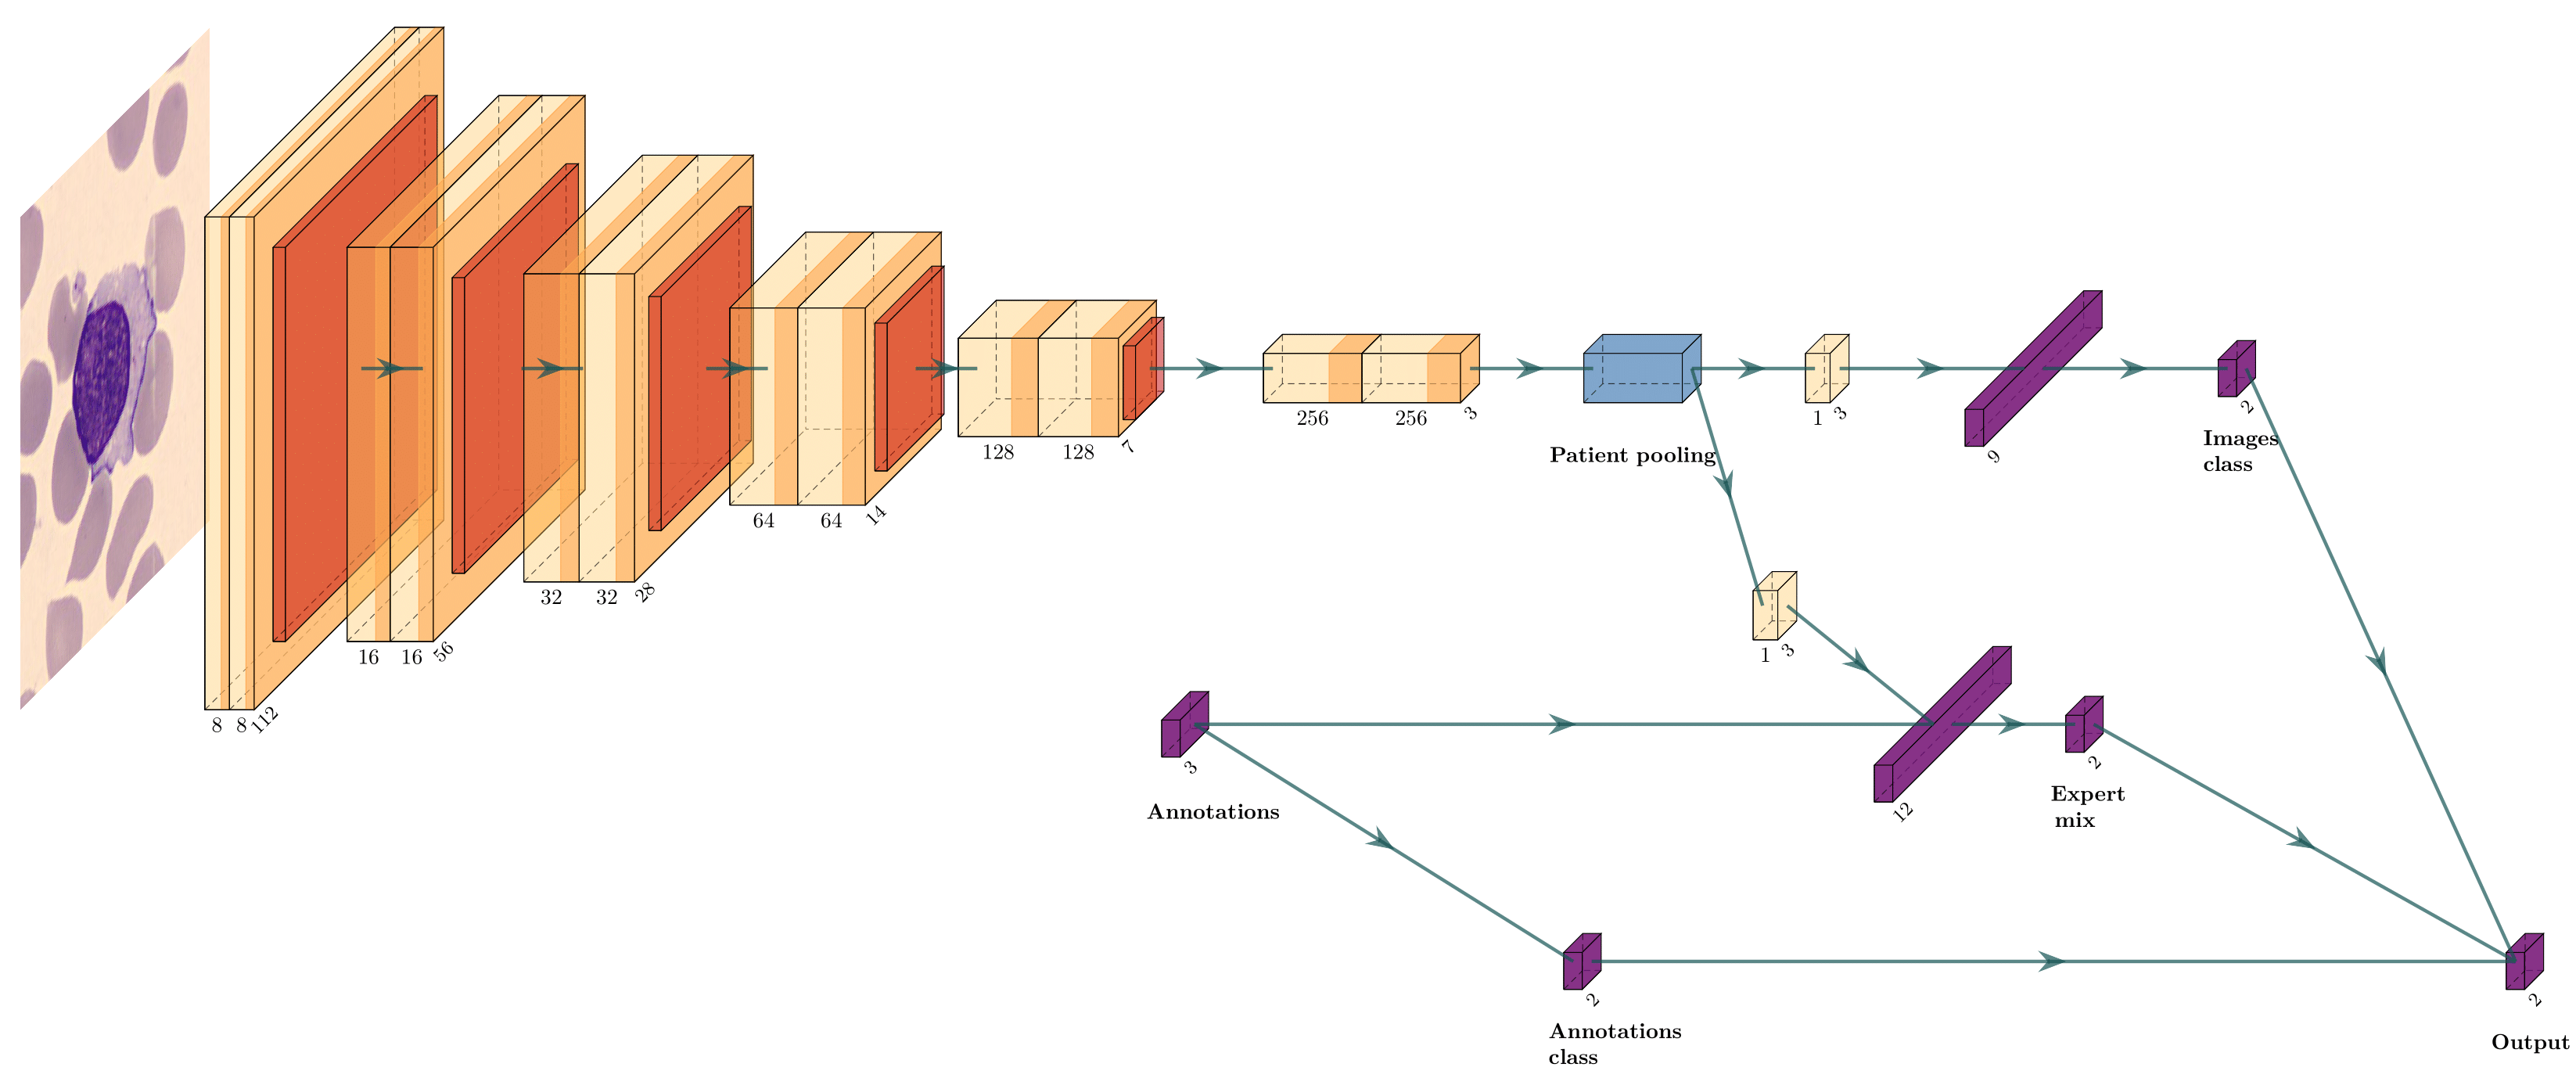
\includegraphics[width=0.9\textwidth]{figures/moe.png}
    \vspace*{-\baselineskip}
    \caption{Mixture of experts architecture. The model is composed of a feature extractor that operates on images, which are then mean-pooled by patient. The other components are a classifier based on extracted feature maps, a classifier based on patient annotations, and a gating network that decides how to mix the two classifiers.}
    \label{fig:mixture_of_experts}
\end{figure}

\section{Model tuning and comparison}
\label{sec:evaluation}

\subsection{Data preprocessing}

\paragraph*{Annotations}
The first step in the challenge is an analysis of the data distributions to make correct preprocessing and architectural choices. In figure \ref{fig:train_test_histograms}, we observe that the training and test datasets have similar enough distributions of their features (taking into account the small number of samples 163 training samples and 42 testing samples).

\begin{figure}[h]
    \centering
    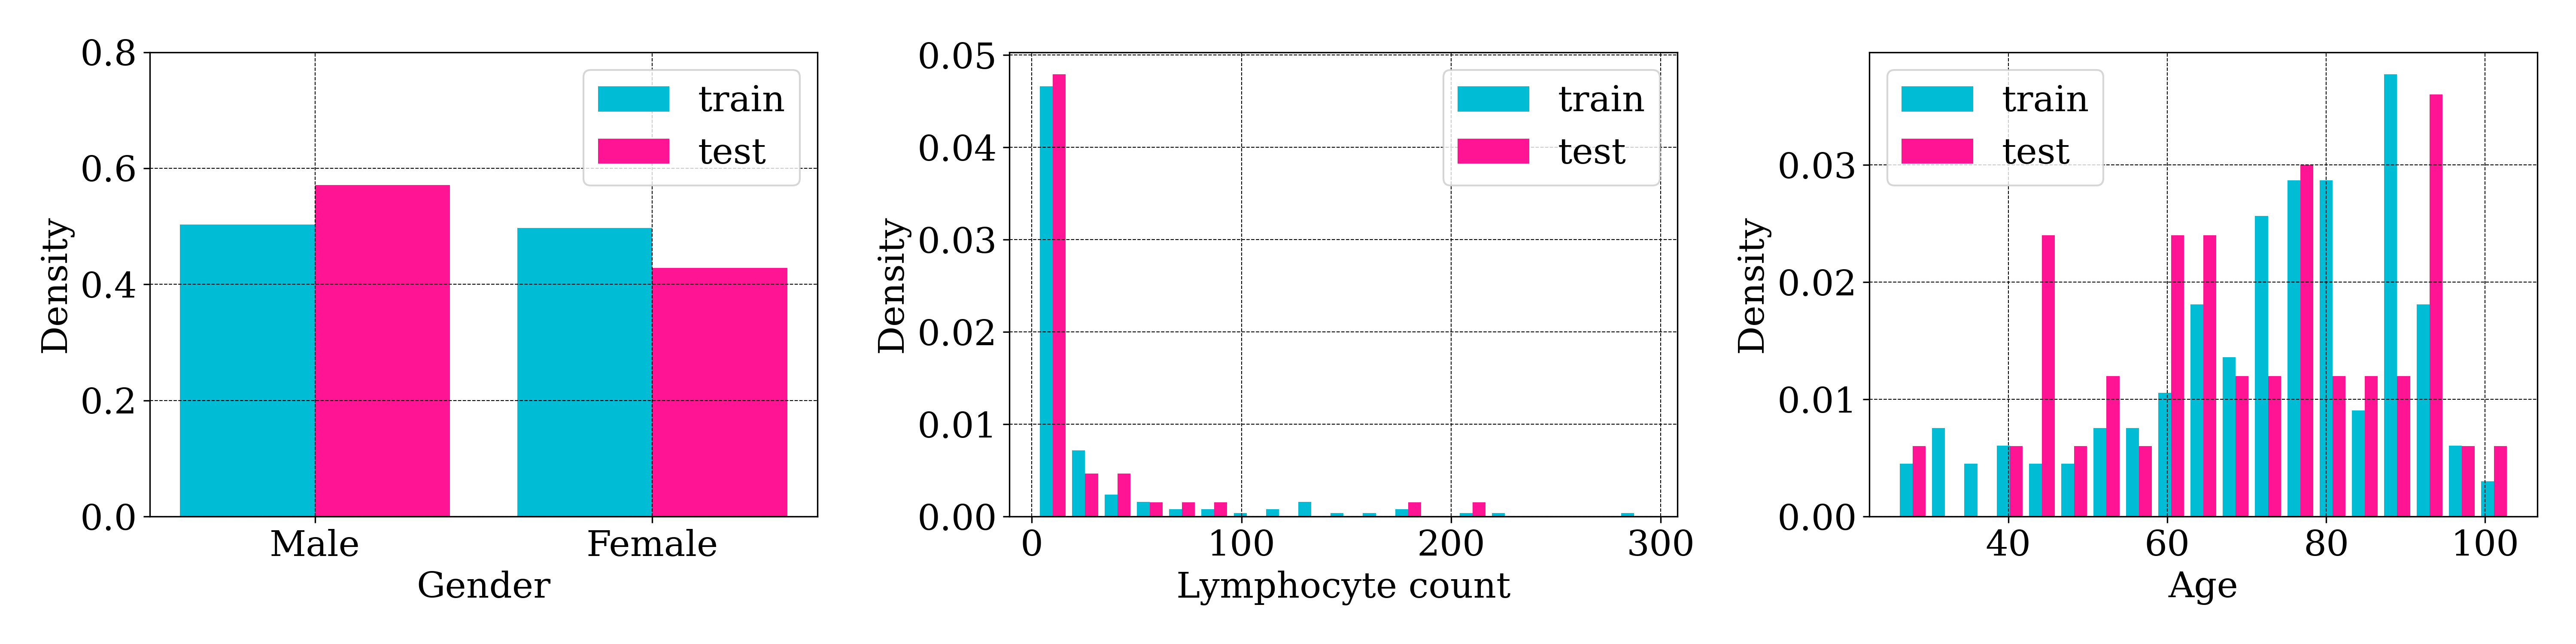
\includegraphics[width=0.9\textwidth]{figures/train_test_histograms.png}
    \vspace*{-\baselineskip}
    \caption{Histograms of the training and test datasets.}
    \label{fig:train_test_histograms}
\end{figure}

On figure \ref{fig:positive_negative_histograms}, we observe the distribution of the positive and negative classes in the training dataset. While gender does not seem to be a good predictor of the negative (reactive) or positive (malignant) class, a high lymphocyte count seems to be a good indicator of malignant lymphocytosis. The malignant nature is also more prevalent in older patients.

\begin{figure}[h]
    \centering
    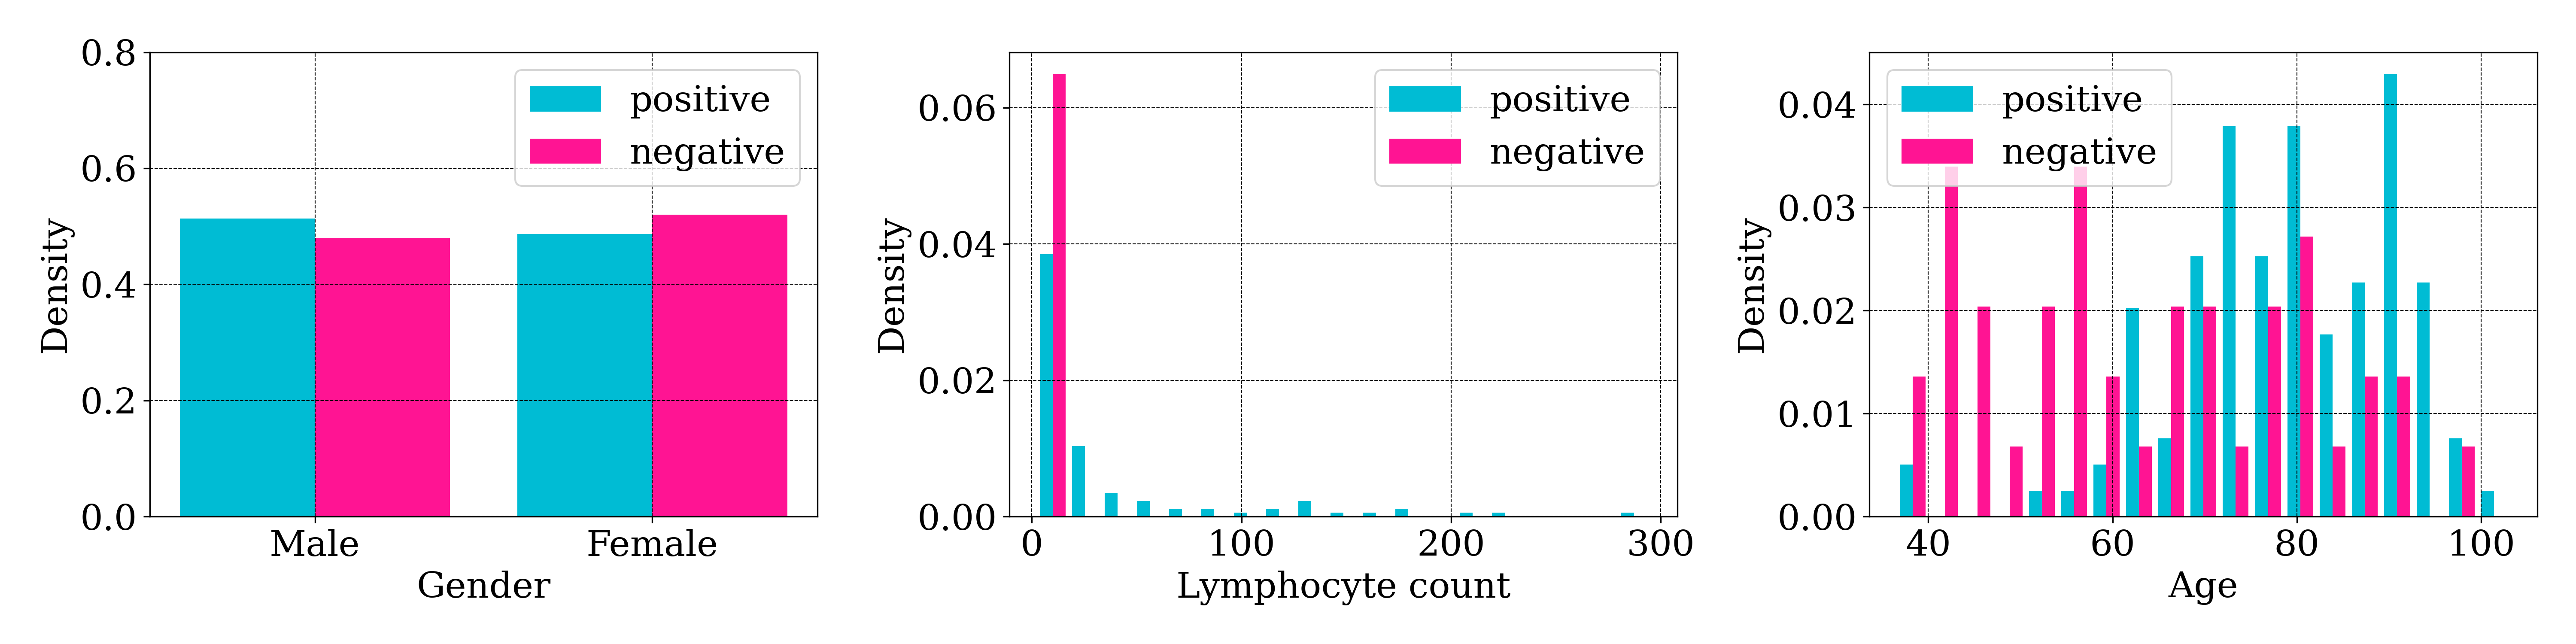
\includegraphics[width=0.9\textwidth]{figures/positive_negative_histograms.png}
    \vspace*{-\baselineskip}
    \caption{Histograms of the positive and negative classes in the training dataset.}
    \label{fig:positive_negative_histograms}
\end{figure}

The imbalance between the positive and negative classes (113 vs. 50) justifies the use of a \textbf{stratified split} of the training dataset between training and validation sets, i.e. we split the dataset so that the proportions of positive and negative classes are the same in the training and validation sets. We also normalize the lymphocyte count and age features to be between 0 and 1.

\paragraph*{Images}
Each patient is associated with a set of images, which are all of size $224\times224$ pixels. For every deep learning model, we apply the following preprocessing steps, motivated by experimental results:
\begin{enumerate}
    \setlength\itemsep{0em}
    \item \textbf{Normalization}: each image is normalized with standard normalization values (mean = [0.485, 0.456, 0.406], std = [0.229, 0.224, 0.225]).
    \item \textbf{Cropping}: in most images, the relevant information is located in the center of the image (the images are taken by an automatic microscope which centers the cells). We crop the images to a size of 112x112 pixels, which gets rid of 75\% of the pixels while keeping the relevant information.
    \item \textbf{Segmentation} (optional): we applied a segmentation algorithm based on a K-means clustering of the saturation channel of the image. While the segmentation algorithm works well enough, it does not seem to improve the performance of the models, so we do not use it in the final models (figure \ref{fig:segmentation}).
\end{enumerate}

\subsection{Training}

We train all models with the Adam optimizer (weight decay of $0.0005$, $(\beta_1,\beta_2)=(0.9, 0.999)$) and a learning rate scheduler that decays the learning rate by $0.975$ at each epoch. Each model is trained for 200 epochs. Note that we perform pseudo early stopping based on the balanced validation accuracy (i.e. the final model is the one that has the best balanced accuracy over all epochs). The initial learning rates and batch sizes are detailed in table \ref{tab:training_parameters}.
\begin{table}[H]
    \begin{center}
        \begin{tabular}{|c|c|c|c|}
            \hline
            \textbf{Model}     & \textbf{Learning rate} & \textbf{Batch size} \\
            \hline
            Baseline           & 0.001                  & 128 (images)        \\
            \hline
            Mixture of experts & 0.0001                 & 8 (patients)        \\
            \hline
        \end{tabular}
    \end{center}
    \vspace*{-\baselineskip}
    \caption{Training parameters.}
    \label{tab:training_parameters}
\end{table}
We use a cross-entropy loss with a weight of $2$ for the positive class and $1$ for the negative class, which is motivated by the application of the model in a medical context where false negatives are more costly than false positives.

\subsection{Results}

We present intermediary results for the three main architectures in table \ref{tab:results}, with the same validation split for all models. While all models have a similar training accuracy, the validation accuracies and test accuracies vary greatly. We believe that 1. there is not enough data to reach a good generalization, and 2. there is not enough data to make meaningful splits.

\begin{table}[H]
    \begin{center}
        \resizebox{\columnwidth}{!}{
            \begin{tabular}{|c|c|c|c|}
                \hline
                \textbf{Model}              & \textbf{Training accuracy} & \textbf{Validation accuracy} & \textbf{Test accuracy} \\
                \hline
                Baseline                    & 0.89923                    & 0.73978                      & 0.84935                \\
                \hline
                Unsupervised classification & 0.89027                    & 0.89130                      & 0.78961                \\
                \hline
                Mixture of experts          & 0.883333                   & 0.93478                      & 0.89090                \\
                \hline
            \end{tabular}
        }
    \end{center}
    \vspace*{-\baselineskip}
    \caption{Main balanced accuracy results}
    \label{tab:results}
\end{table}

Given these results, we still chose to use the mixture of experts model for the final submission, as it has the best validation accuracy and the best test accuracy. To test its ability to generalize, we also ran a 5-fold cross-validation on the mixture of experts model (each fold being a stratified split of the training set), and obtained a mean balanced accuracy on the validation sets of $0.94392\pm 0.05$. While these results are promising, we still believe that the model would need more data to really generalize, and while good results are obtained on the public test set, we are not sure that the model will generalize well to the private test set. In particular the training of the mixture of experts model was very unstable, with validation accuracies that could vary greatly from one epoch to the next (figures \ref{fig:loss}, \ref{fig:acc_curve}, \ref{fig:true_negative_rates}, \ref{fig:true_positive_rates}).

\section{Conclusion}

In this work, we have presented a simple baseline model, an unsupervised classification approach, and a mixture of experts model to predict the malignancy of lymphocytosis. The mixture of experts model has the best performance on the validation set and the test set, with a balanced accuracy of $0.89090$. These results are promising, but we believe that we don't capture the full potential of the data, and that many improvements could be made. In particular, while the mixture of experts model has interesting properties, it still relies on a single label for a whole set of images, which contributes to the instability of the training.


\label{sec:conclusion}

\newpage
\bibliography{bibliography}

\appendix

\newpage
\section{Segmentation}

\begin{figure}[H]
    \centering
    {
        \subfigure[Good segmentation][c]{
            \label{fig:good_segmentation}
            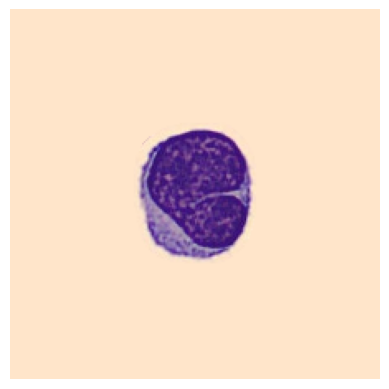
\includegraphics[width=0.25\textwidth]{figures/good_segmentation.png}
        } \qquad
        \subfigure[Bad segmentation][c]{
            \label{fig:bad_segmentation}
            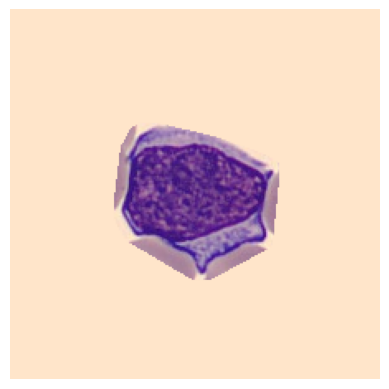
\includegraphics[width=0.25\textwidth]{figures/bad_segmentation.png}
        }
    }
    {\caption{Example of lymphocyte segmentations. On \ref{fig:good_segmentation}, the segmentation is perfect with all the cytoplasm correctly segmented and no left-over pixels. On \ref{fig:bad_segmentation}, the segmentation isn't as great, a lot of blood cell pixels were left to keep all the cytoplasm pixels.\label{fig:segmentation}}}
\end{figure}

\section{Unsupervised classification}

\begin{figure}[H]
    \centering
    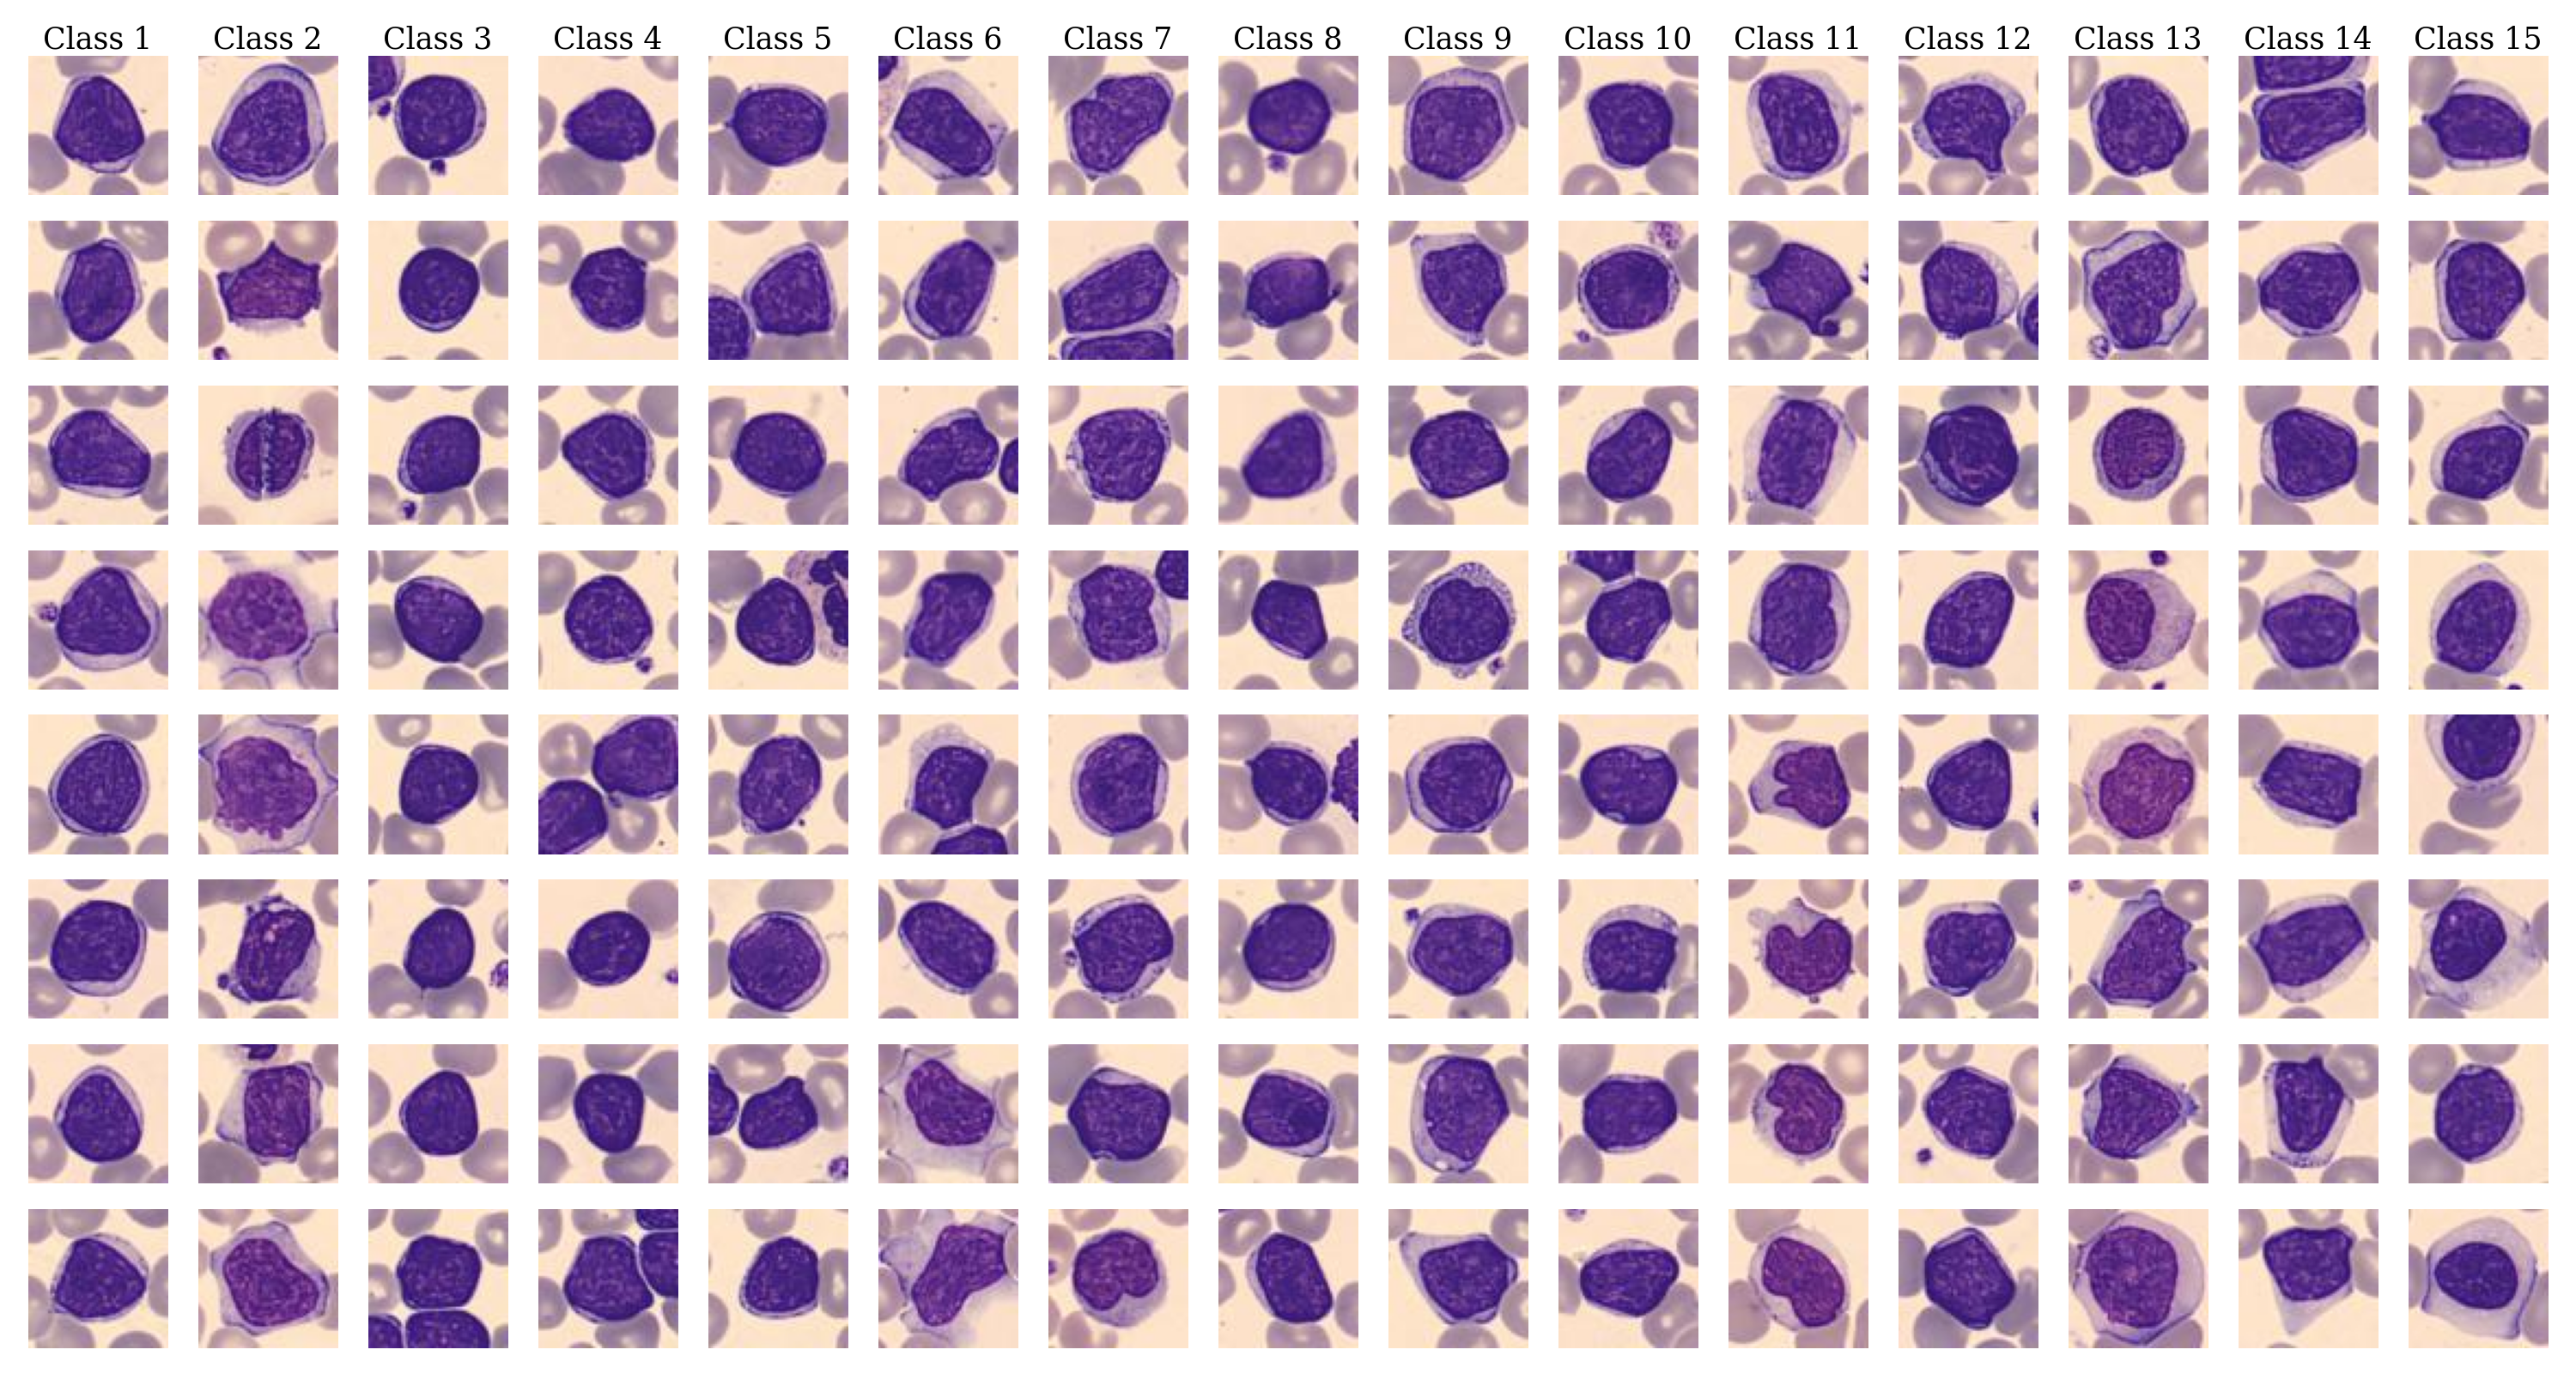
\includegraphics[width=\textwidth]{figures/unsupervised_classification.png}
    \caption{Samples from the 15 classes obtained by unsupervised classification. Each column is a class. We clearly identify some interesting patterns, for instance class 1 is big lymphocytes with medium cytoplasm, class 2 is big lymphocytes with a lot of cytoplasm, class 3 is small lymphocytes with no cytoplasm, etc.}
    \label{fig:unsupervised_classification}
\end{figure}

\begin{figure}[H]
    \centering
    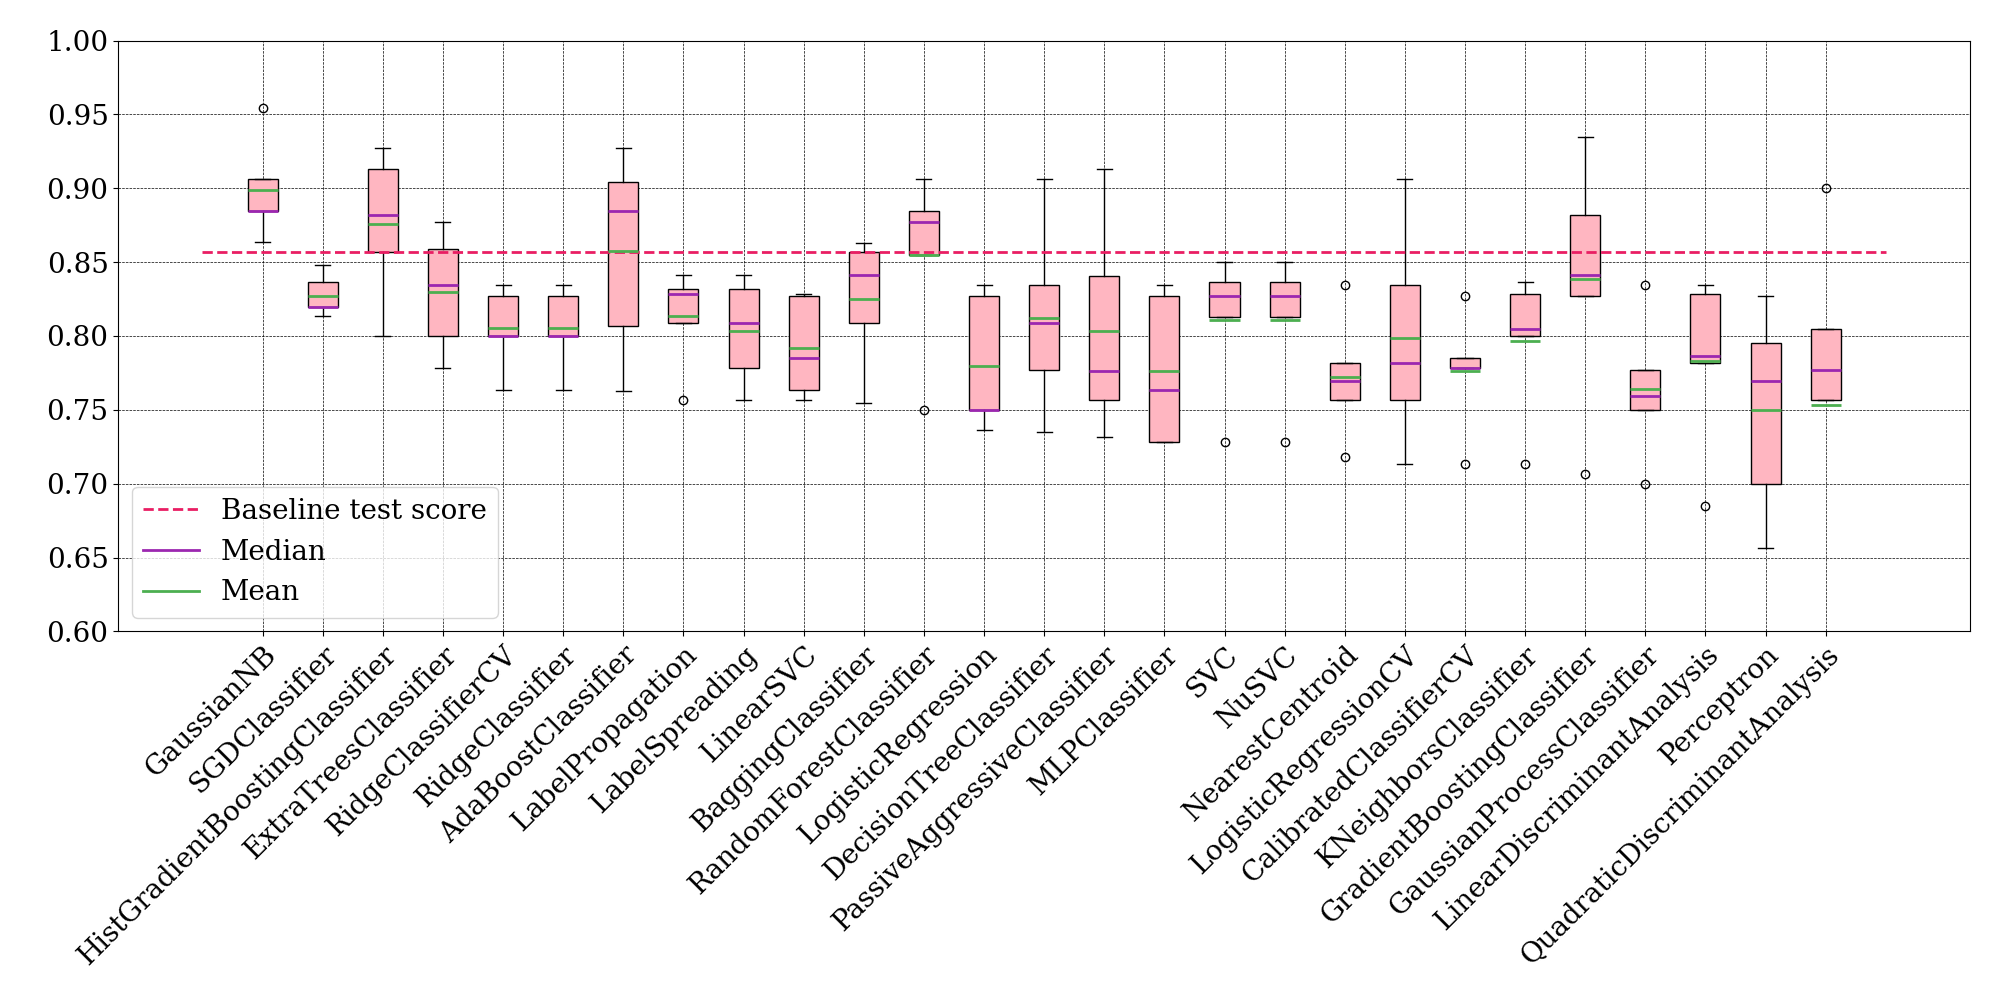
\includegraphics[width=\textwidth]{figures/unsupervised_classification_models.png}
    \caption{Balanced accuracy of different machine learning models on the unsupervised classification features.}
    \label{fig:unsupervised_classification_models}
\end{figure}

\section{Training curves}

\begin{figure}[h]
    \centering
    {
        \subfigure[Training loss][c]{
            \label{fig:train_loss}
            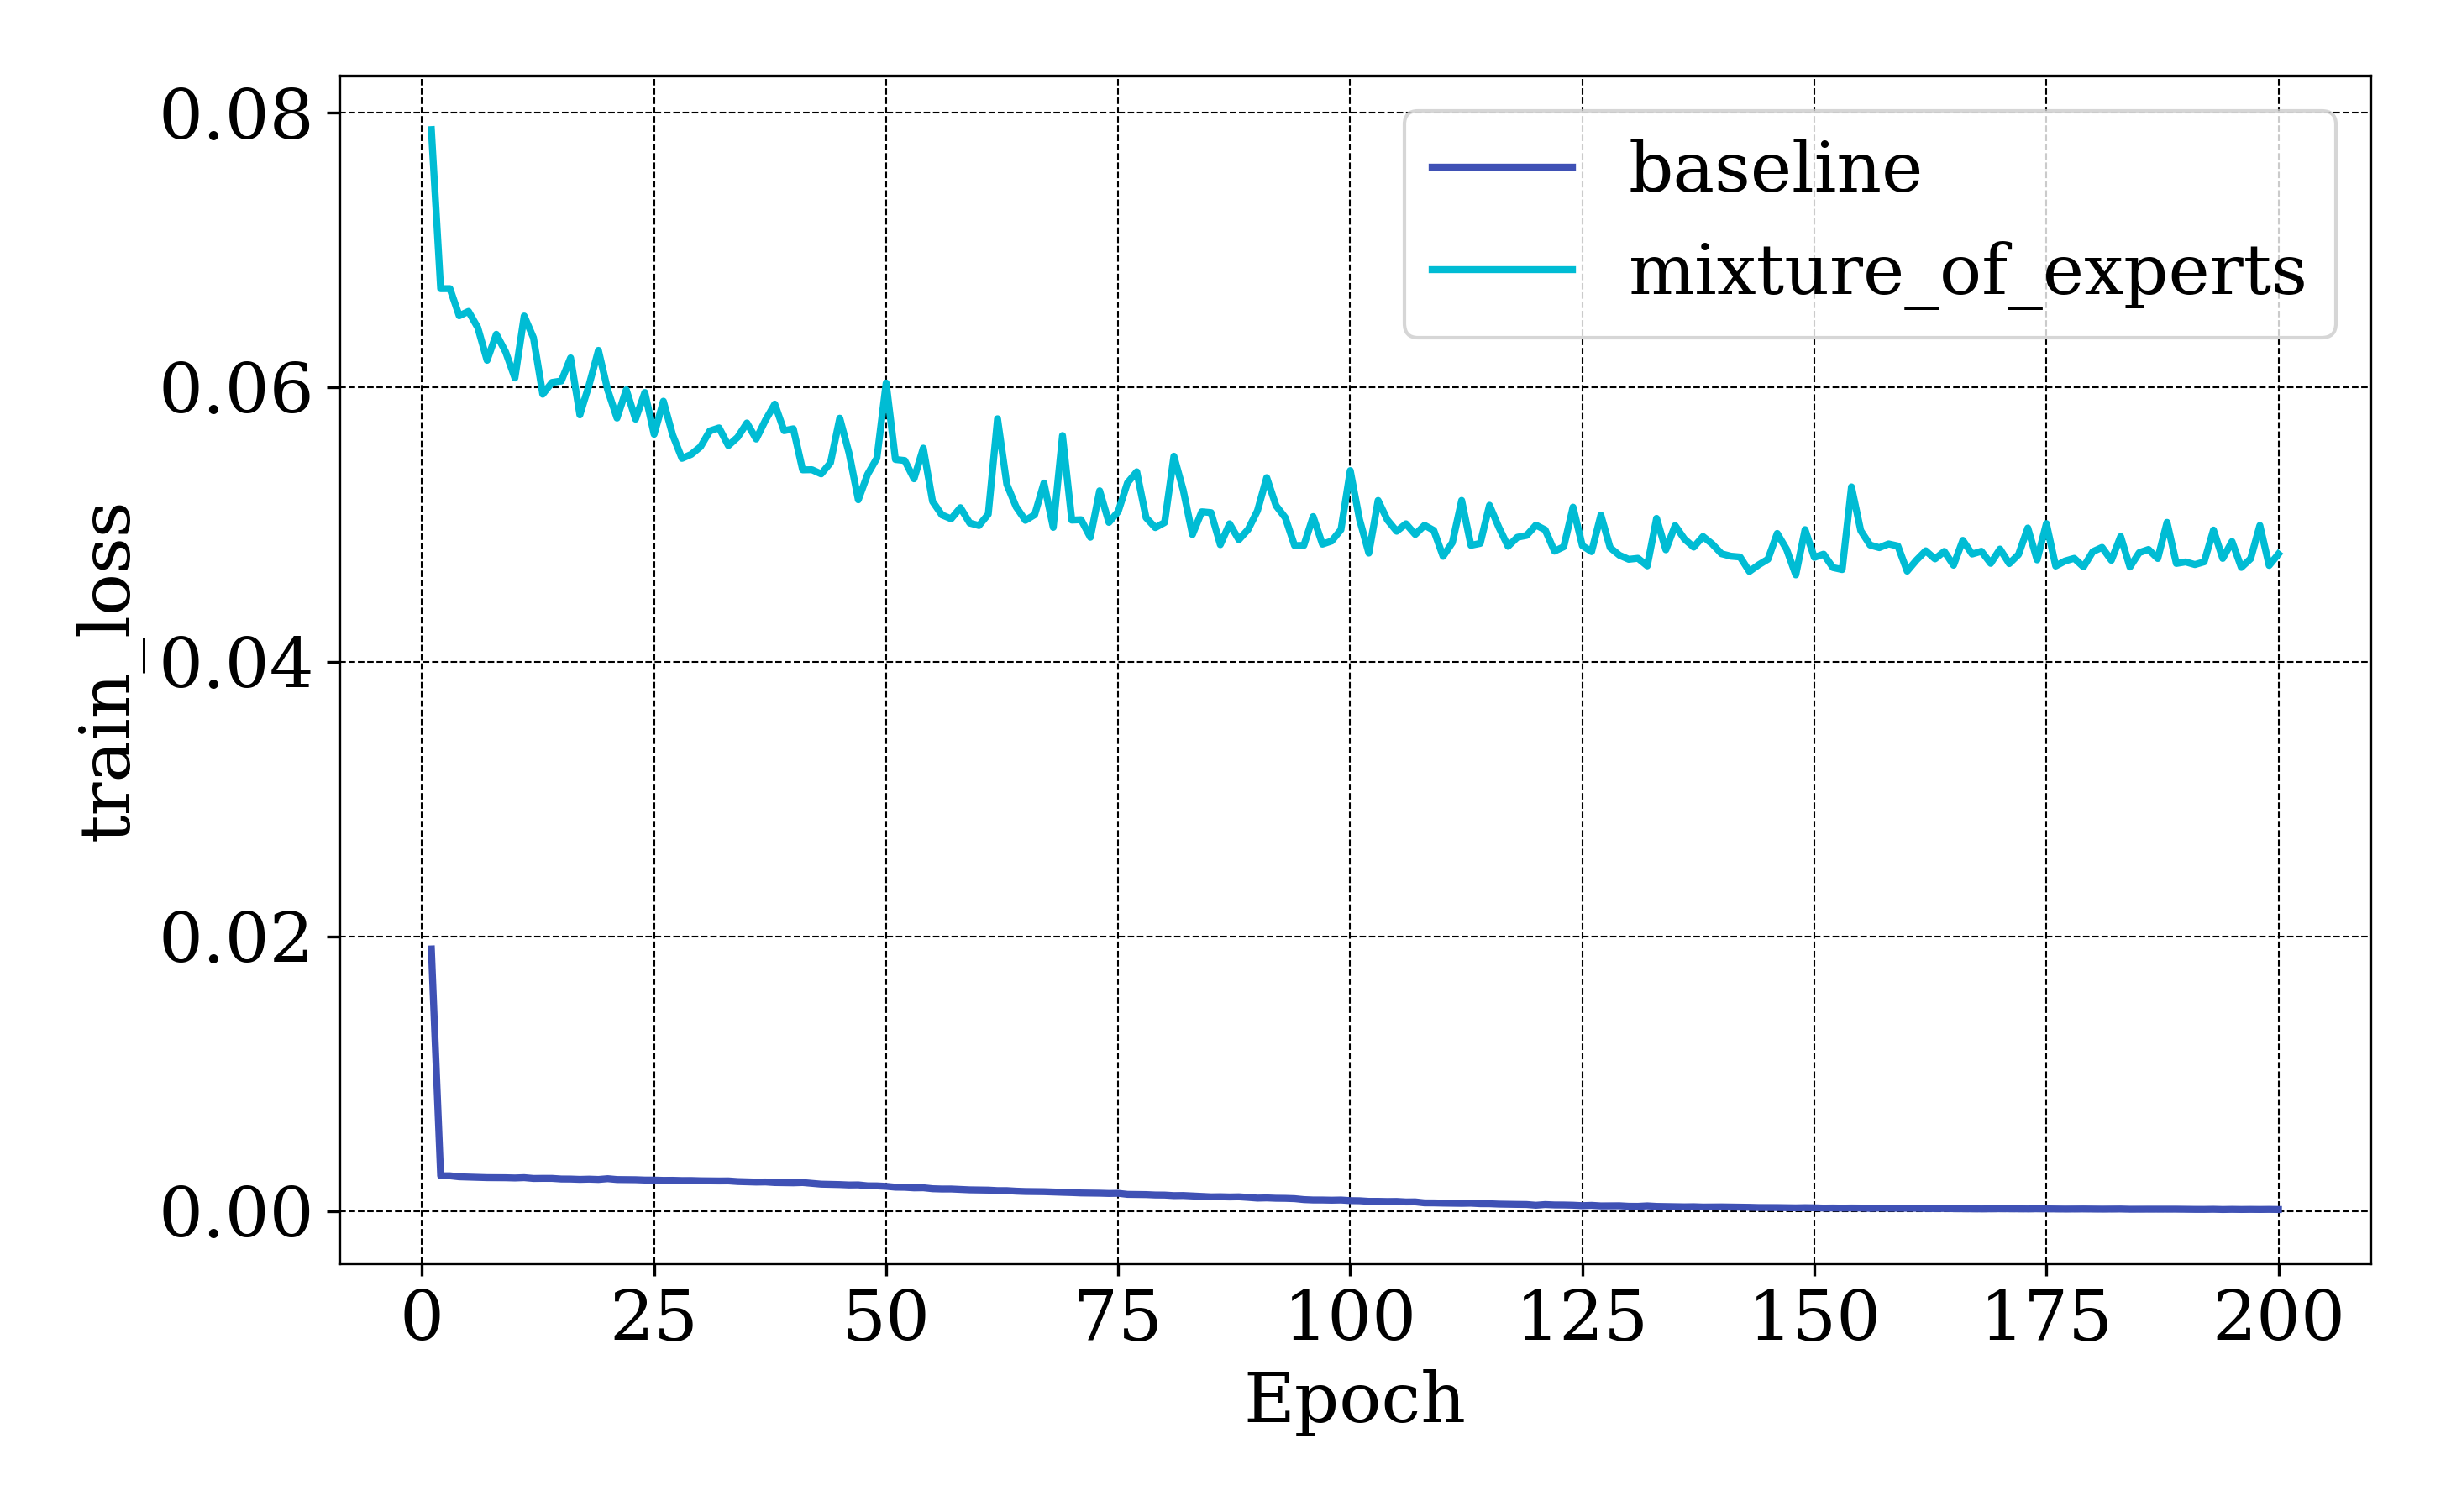
\includegraphics[width=0.45\textwidth]{figures/train_loss.png}
        } \qquad
        \subfigure[Validation loss][c]{
            \label{fig:val_loss}
            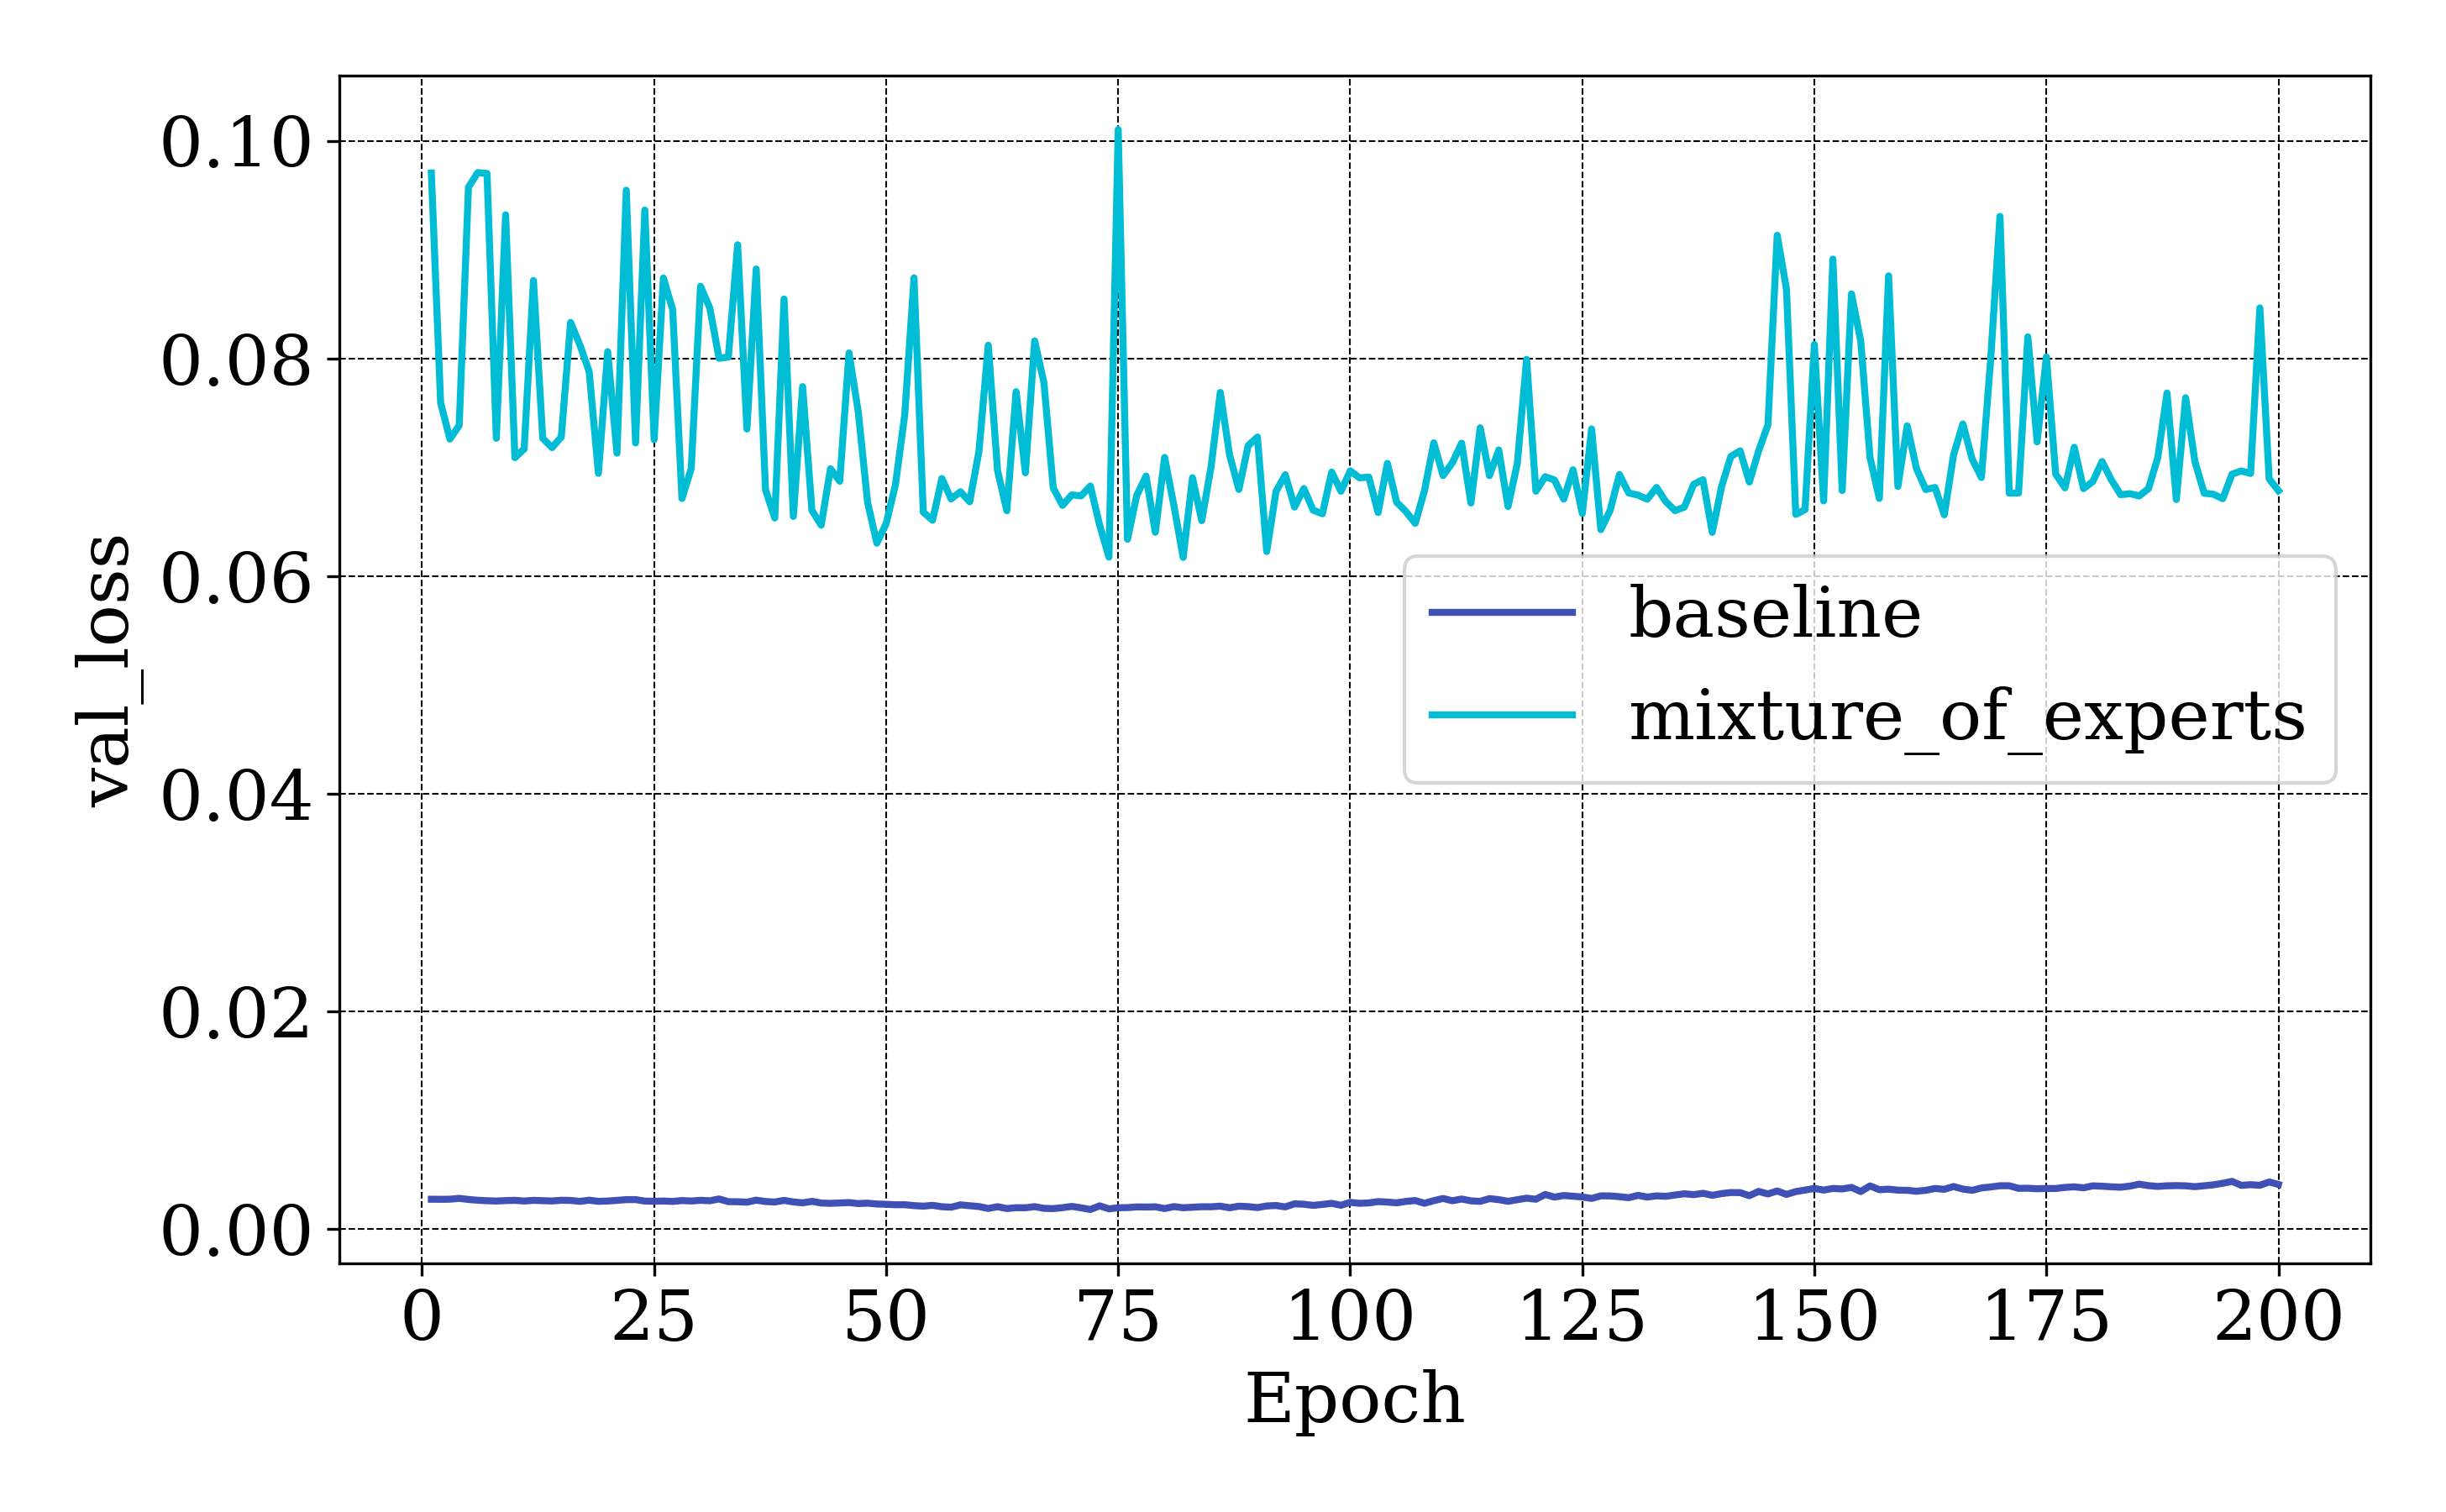
\includegraphics[width=0.45\textwidth]{figures/val_loss.png}
        }
    }
    {\caption{Training and validation loss curves.\label{fig:loss}}}
\end{figure}

\begin{figure}[h]
    \centering
    {
        \subfigure[Training accuracy][c]{
            \label{fig:train_acc}
            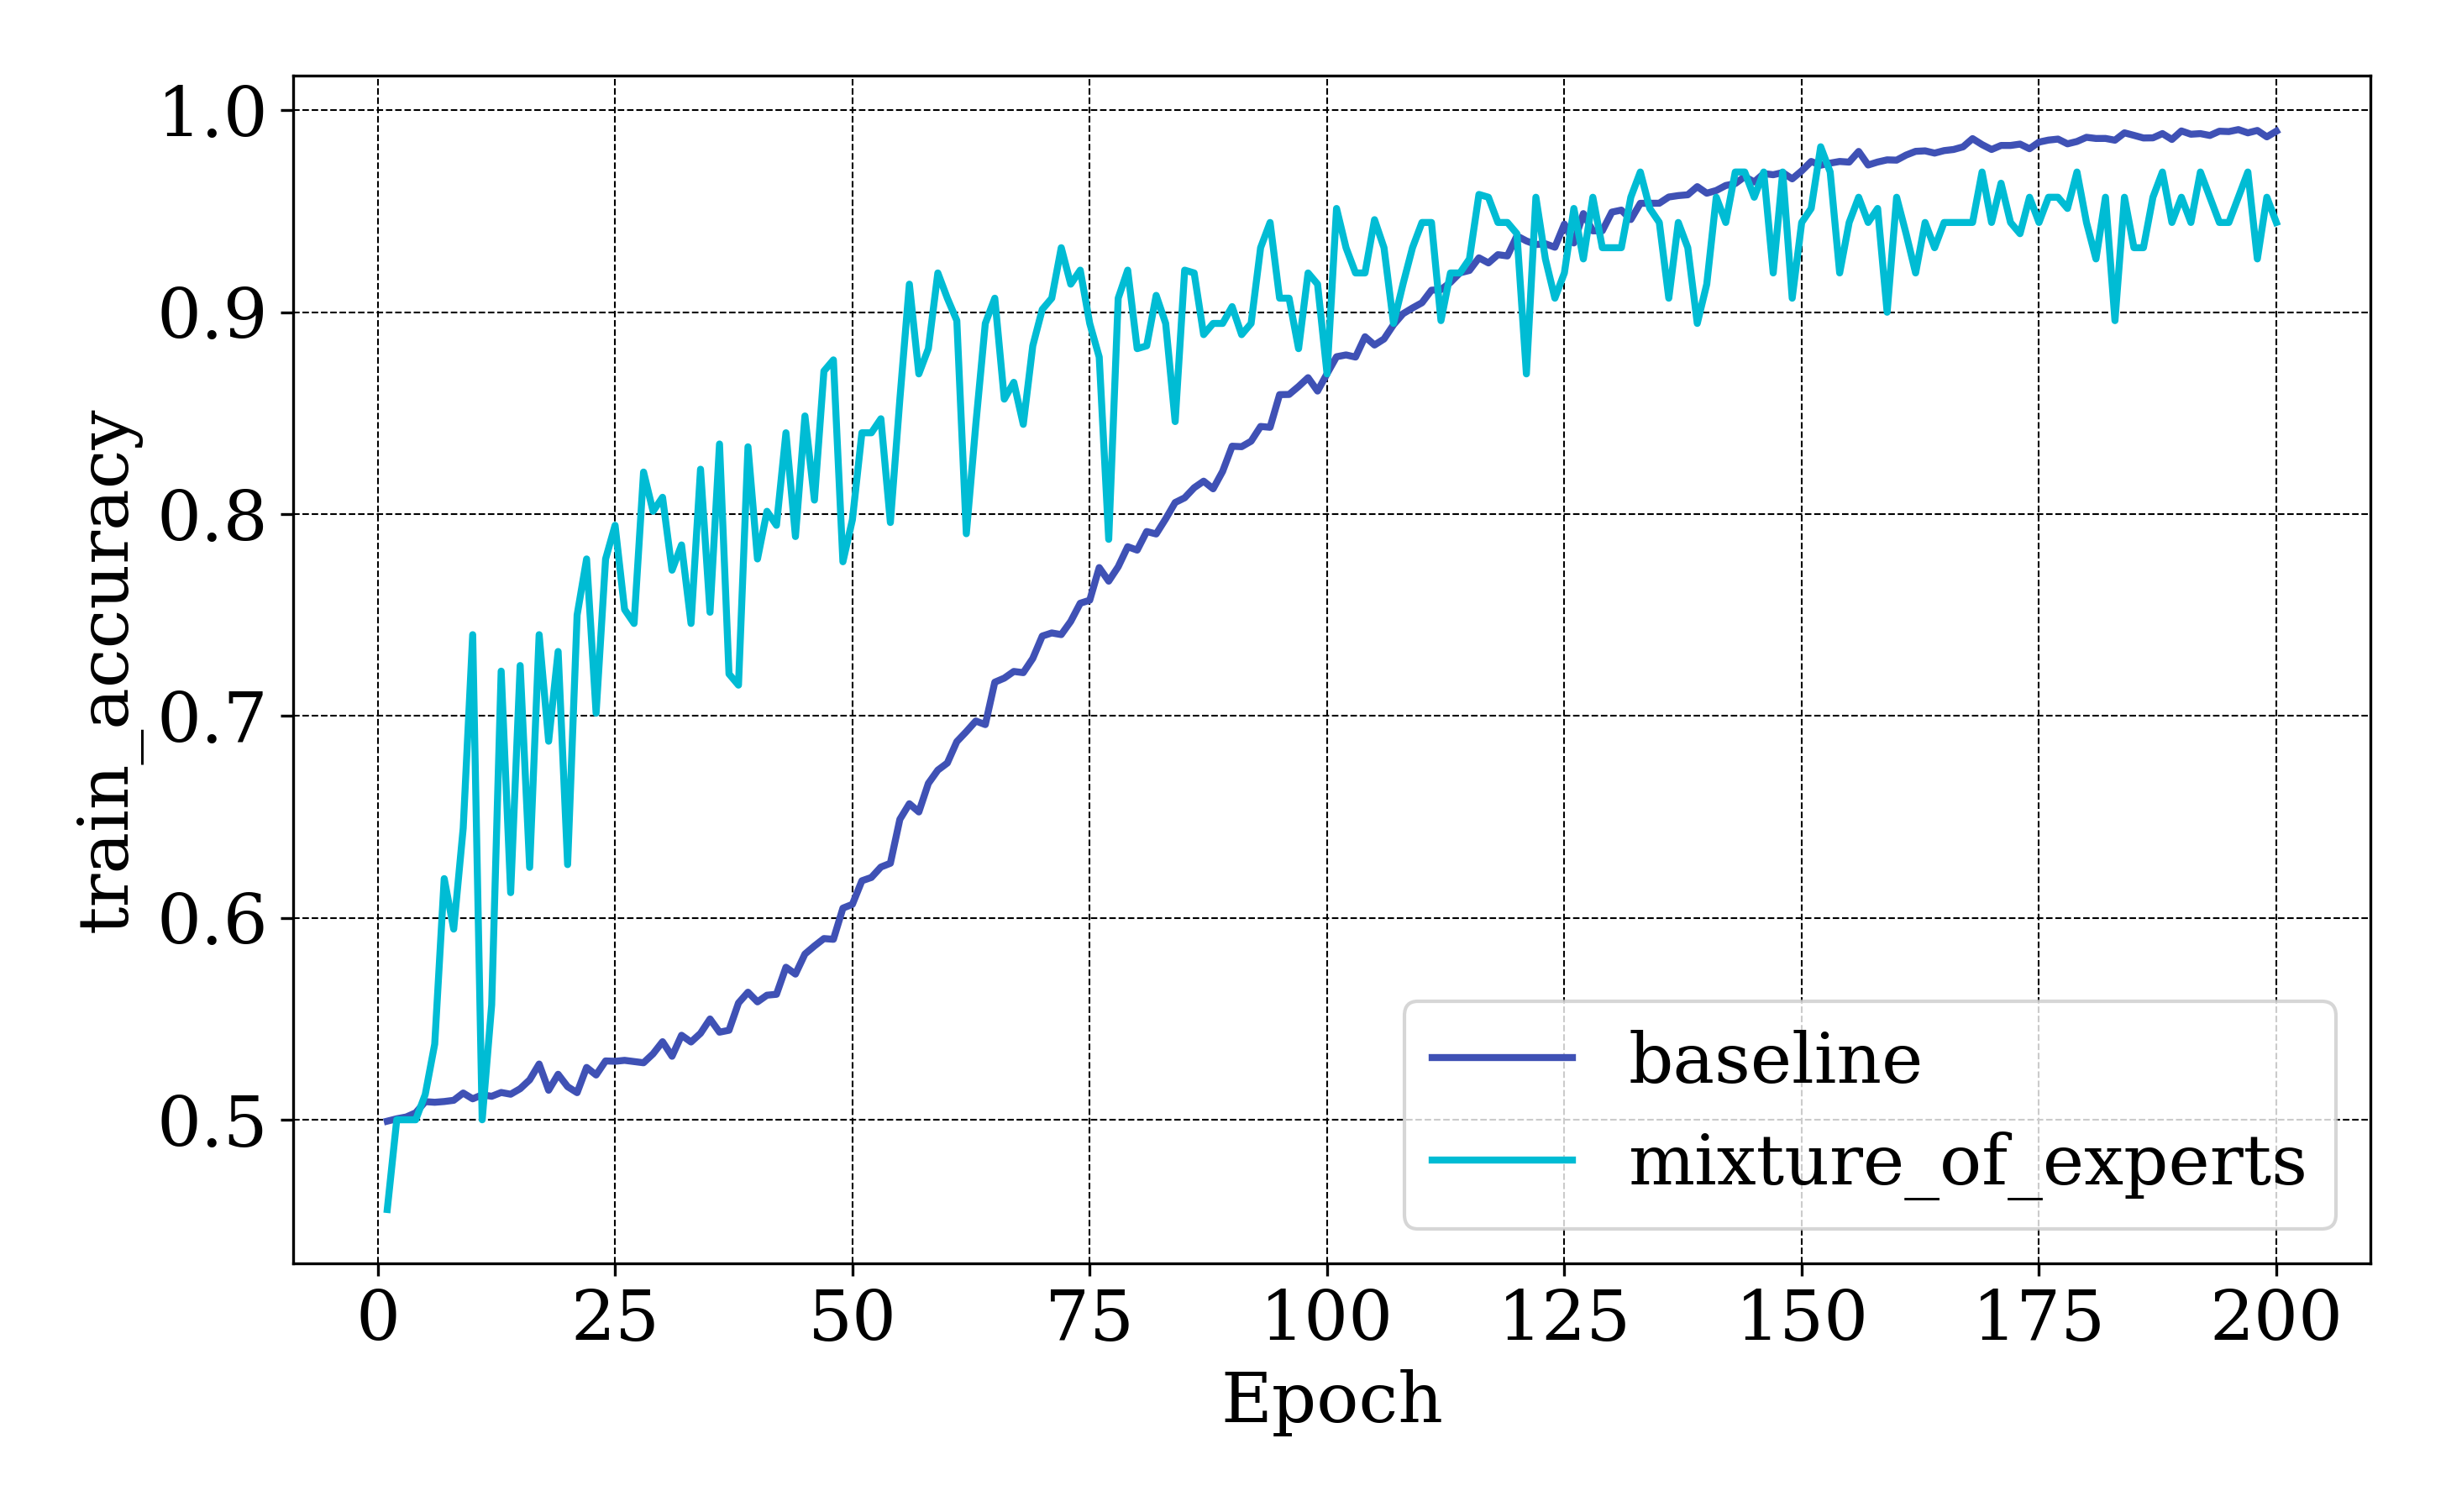
\includegraphics[width=0.45\textwidth]{figures/train_accuracy.png}
        } \qquad
        \subfigure[Validation accuracy][c]{
            \label{fig:val_acc}
            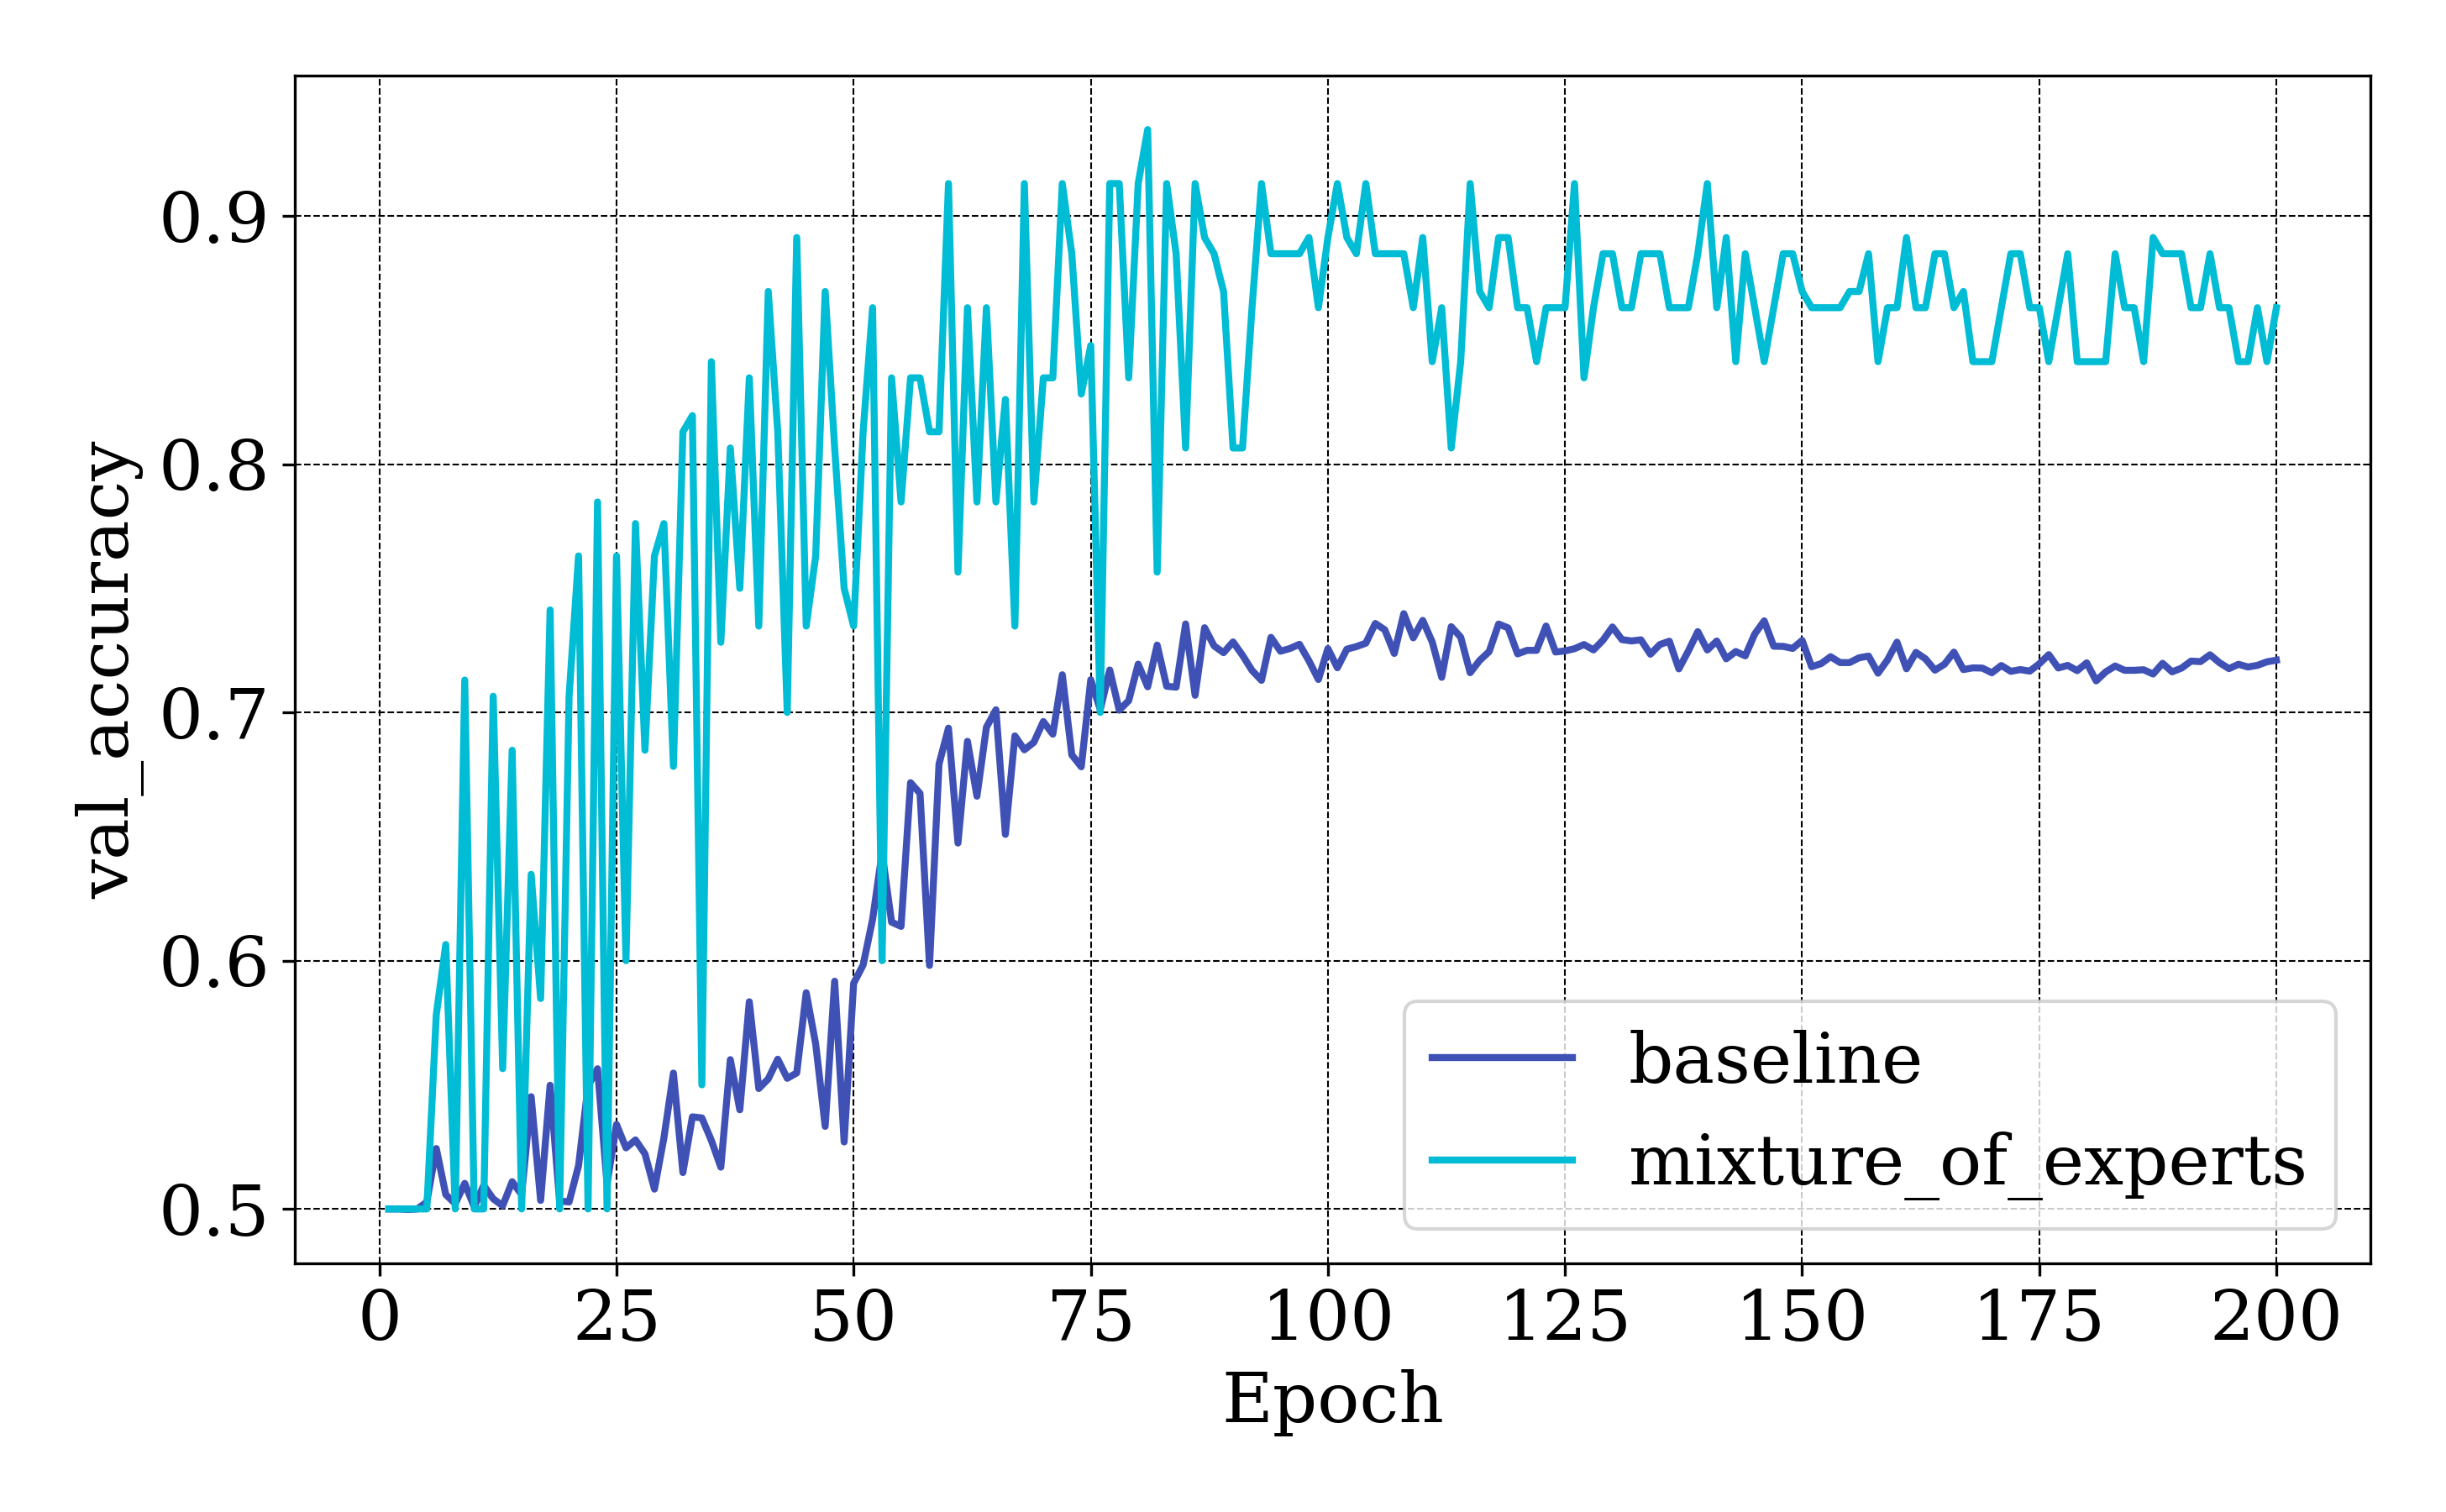
\includegraphics[width=0.45\textwidth]{figures/val_accuracy.png}
        }
    }
    {\caption{Training and validation balanced accuracy curves.\label{fig:acc_curve}}}
\end{figure}

\begin{figure}[h]
    \centering
    {
        \subfigure[Training true negative rate][c]{
            \label{fig:train_true_negative_rates}
            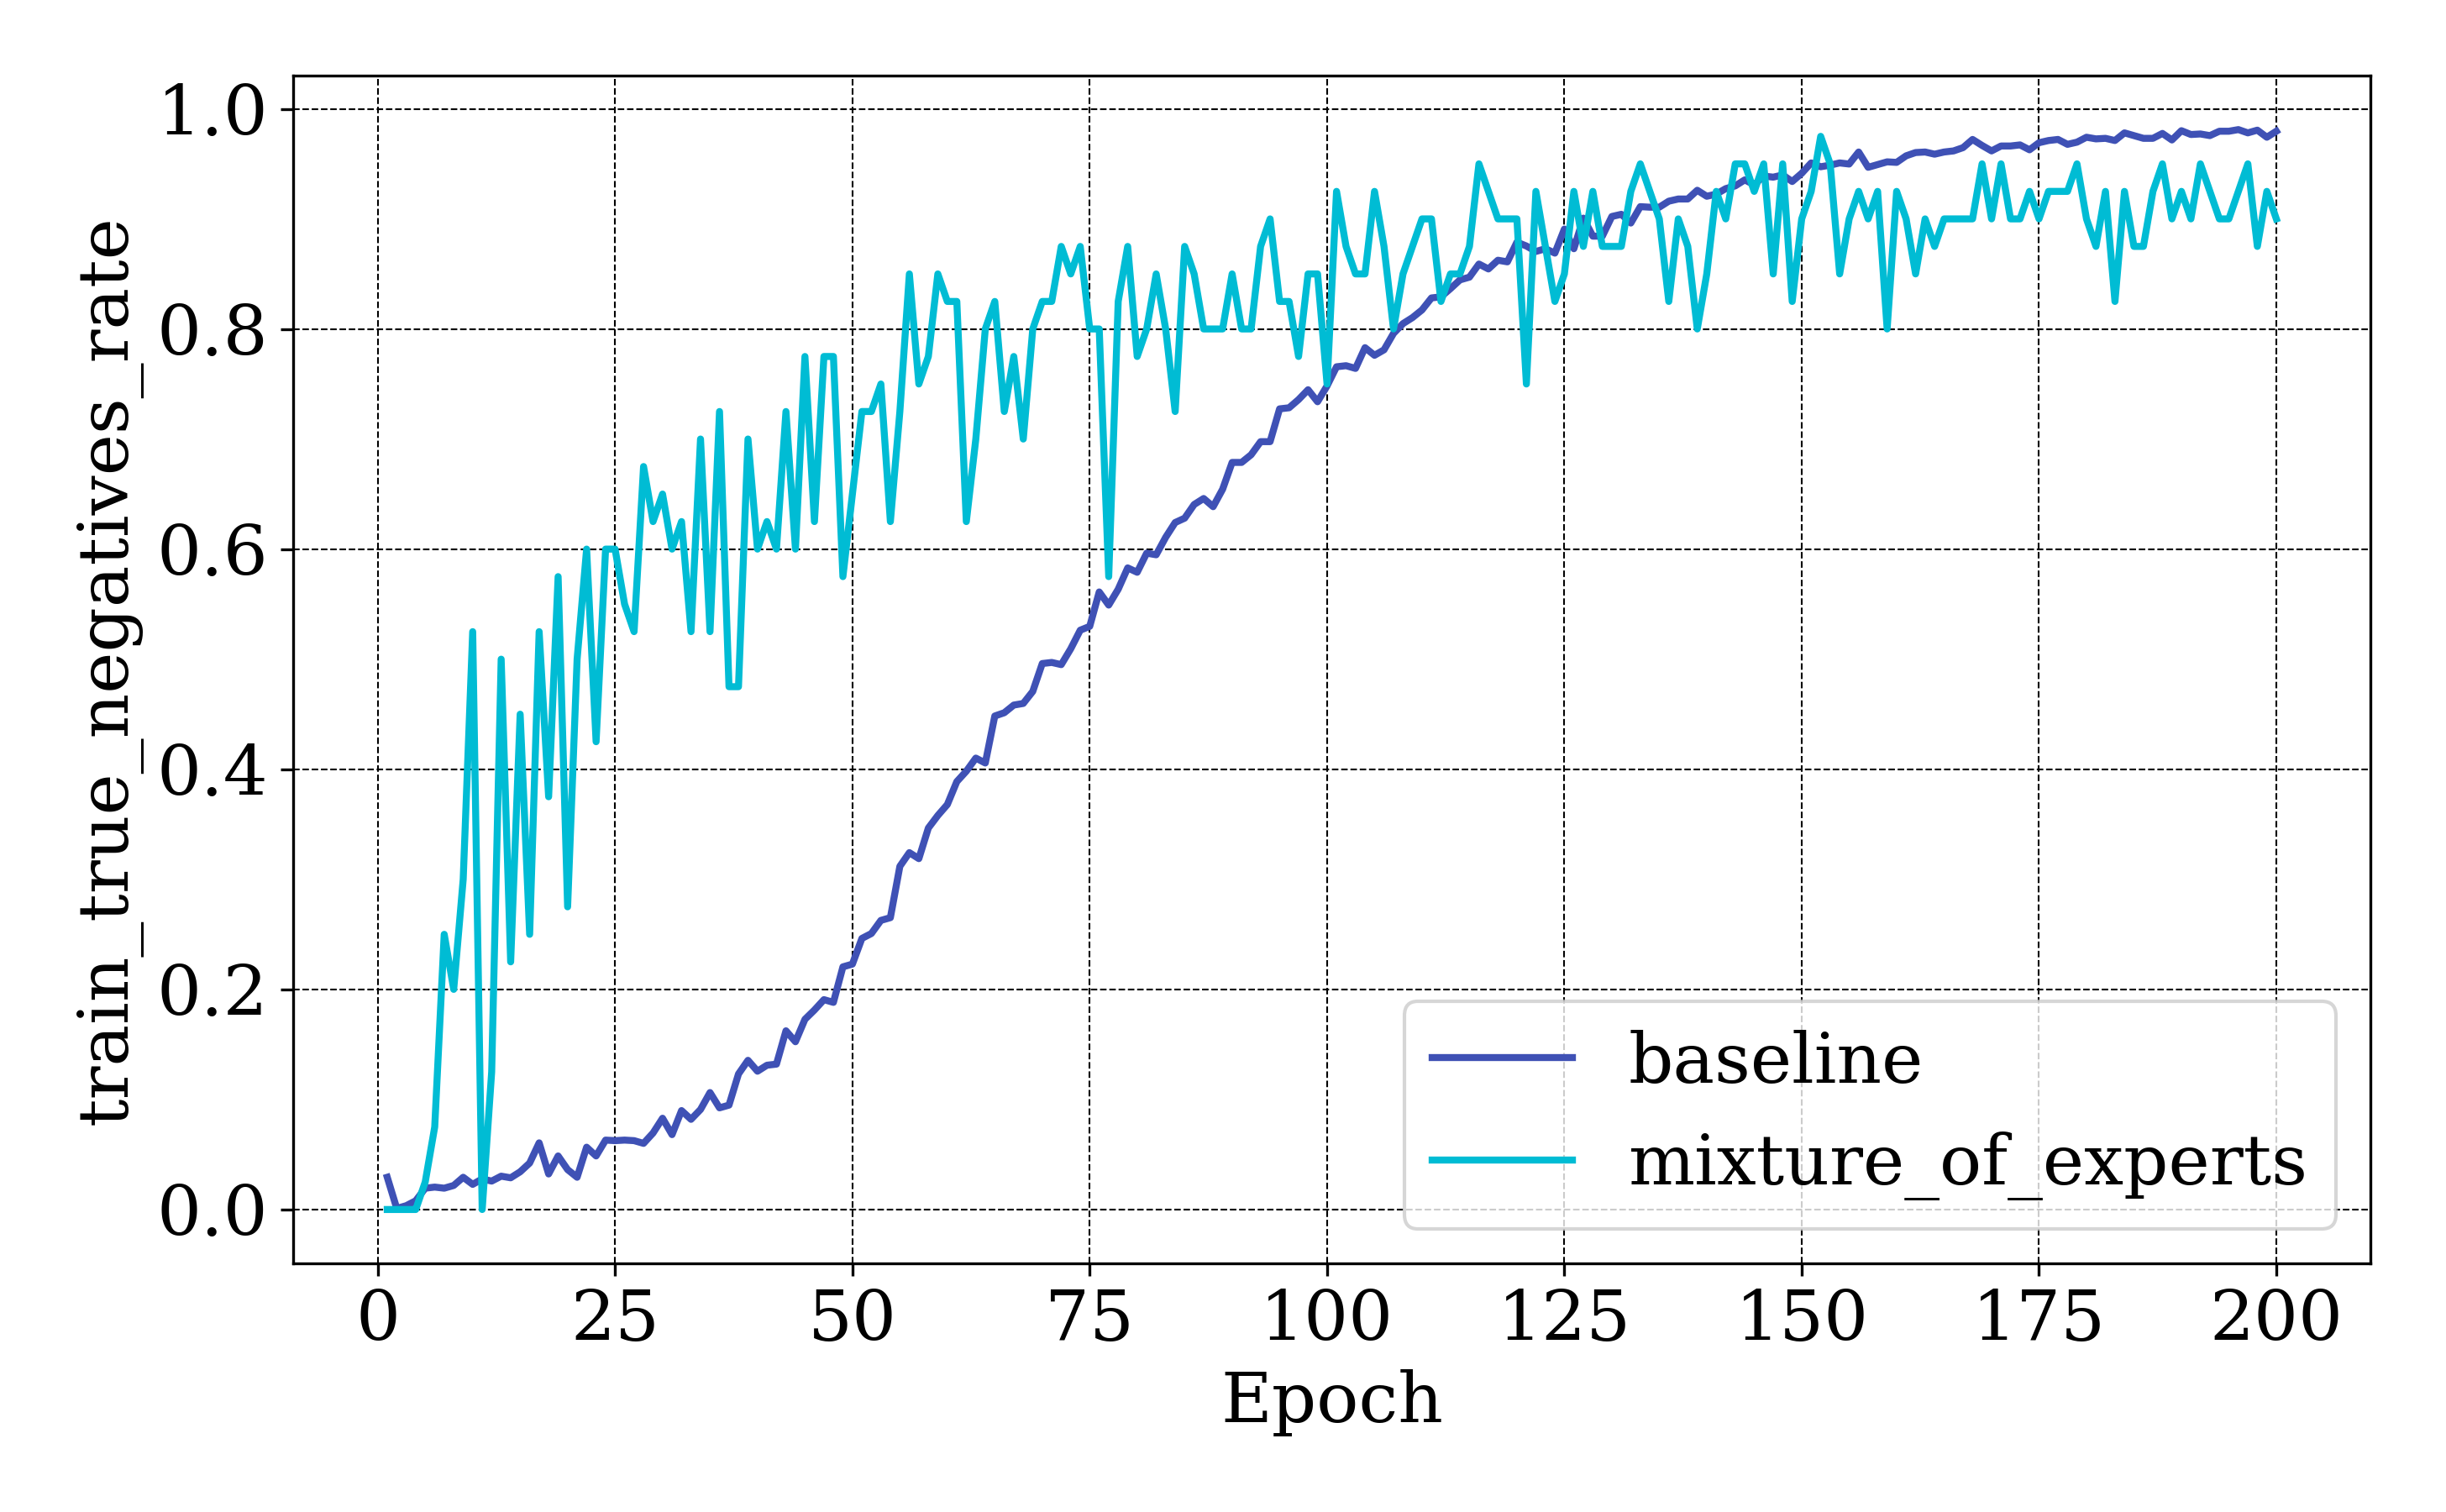
\includegraphics[width=0.45\textwidth]{figures/train_true_negatives_rate.png}
        } \qquad
        \subfigure[Validation true negative rate][c]{
            \label{fig:val_true_negative_rates}
            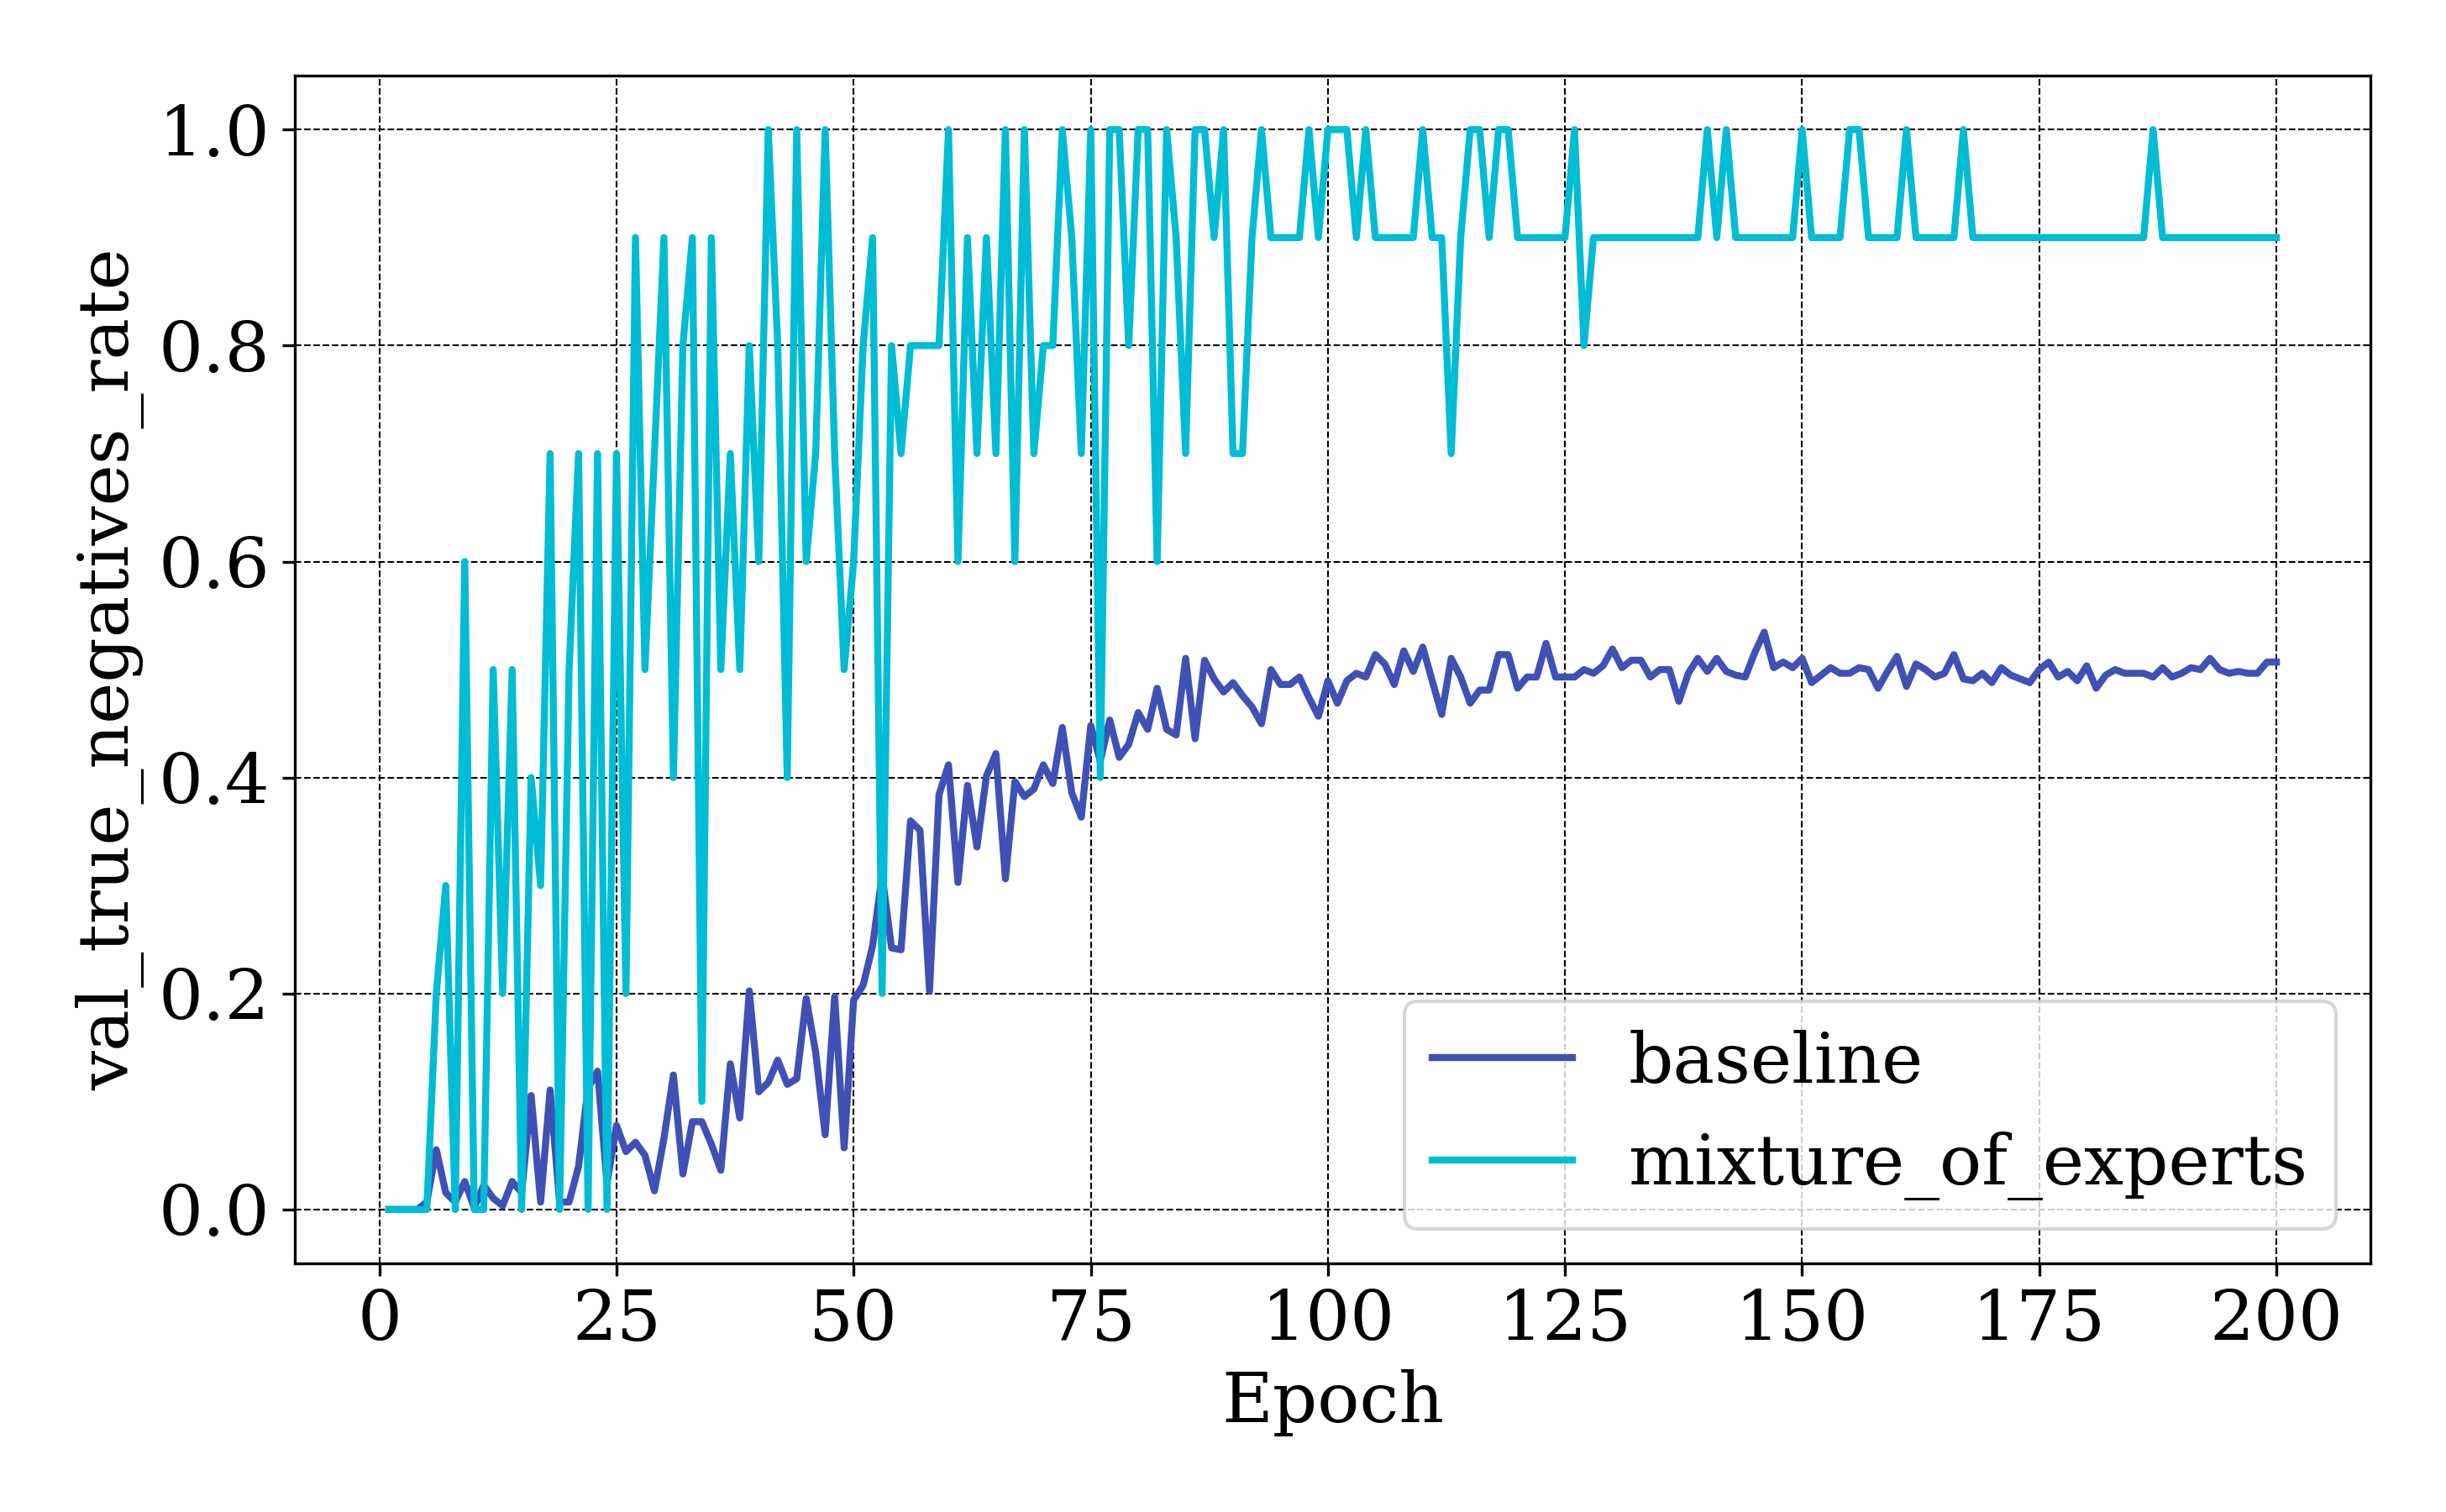
\includegraphics[width=0.45\textwidth]{figures/val_true_negatives_rate.png}
        }
    }
    {\caption{Training and validation true negative rates.\label{fig:true_negative_rates}}}
\end{figure}

\begin{figure}[h]
    \centering
    {
        \subfigure[Training true positive rate][c]{
            \label{fig:train_true_positive_rates}
            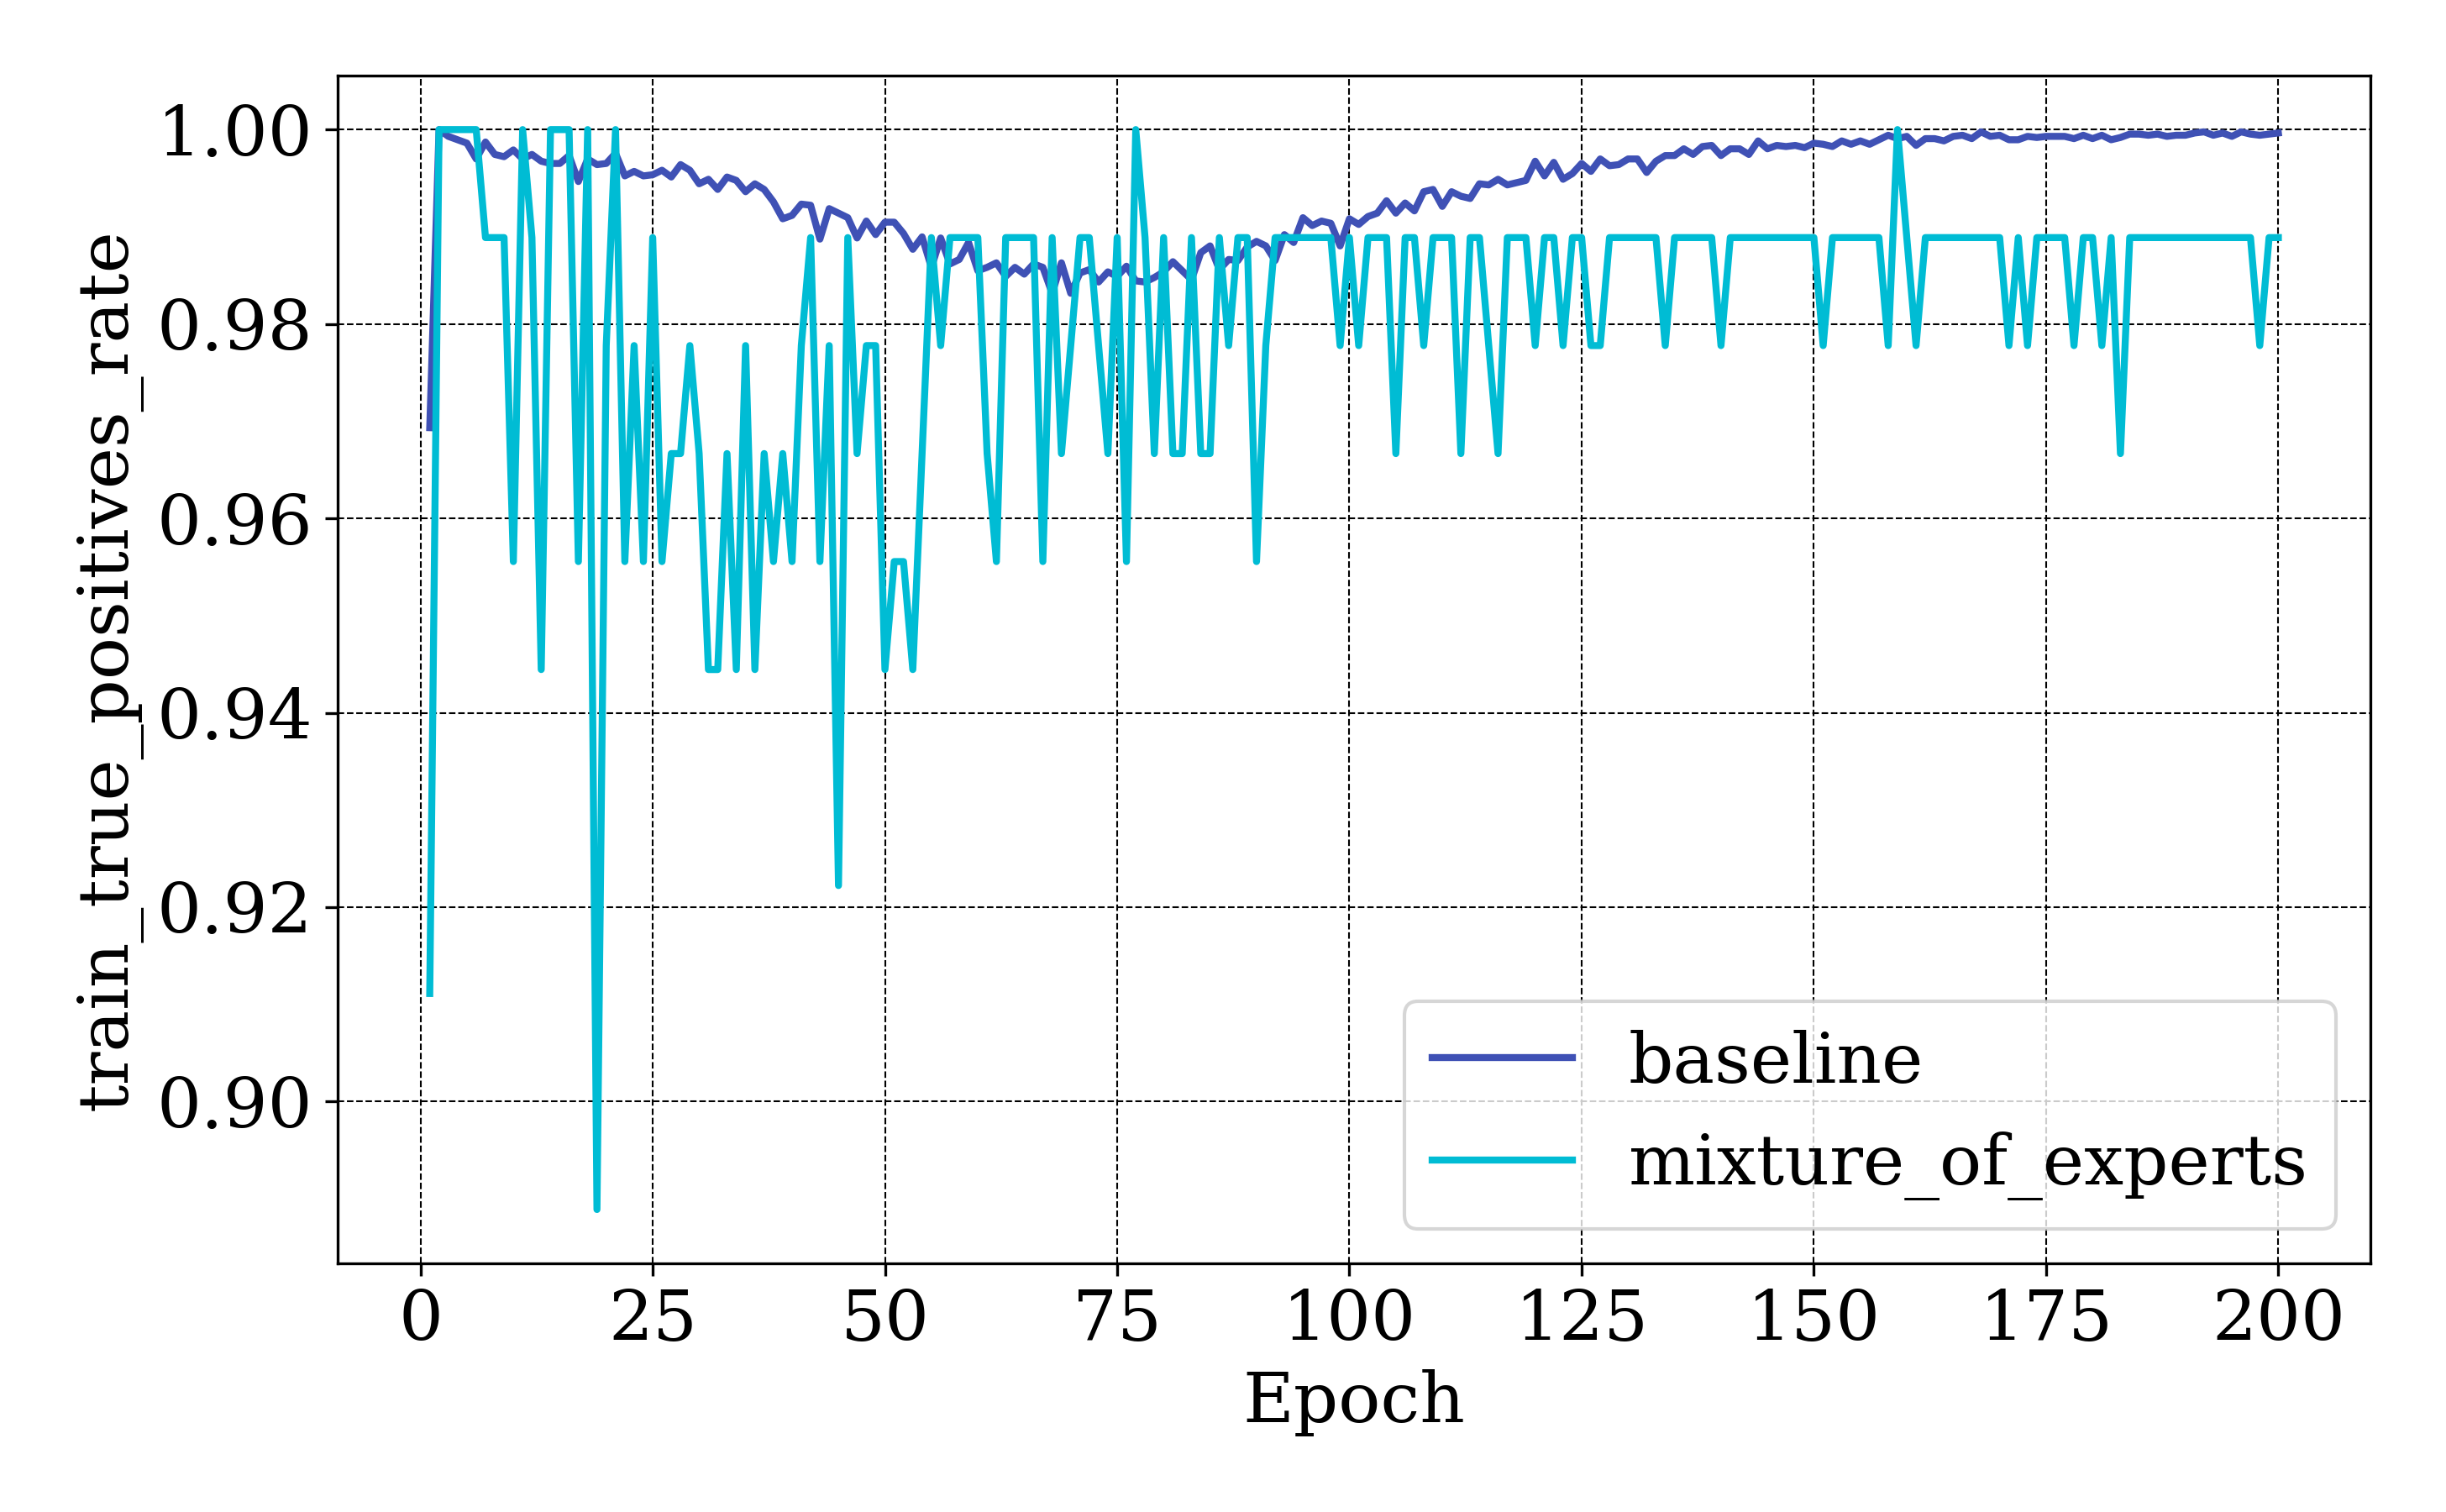
\includegraphics[width=0.45\textwidth]{figures/train_true_positives_rate.png}
        } \qquad
        \subfigure[Validation true positive rate][c]{
            \label{fig:val_true_positive_rates}
            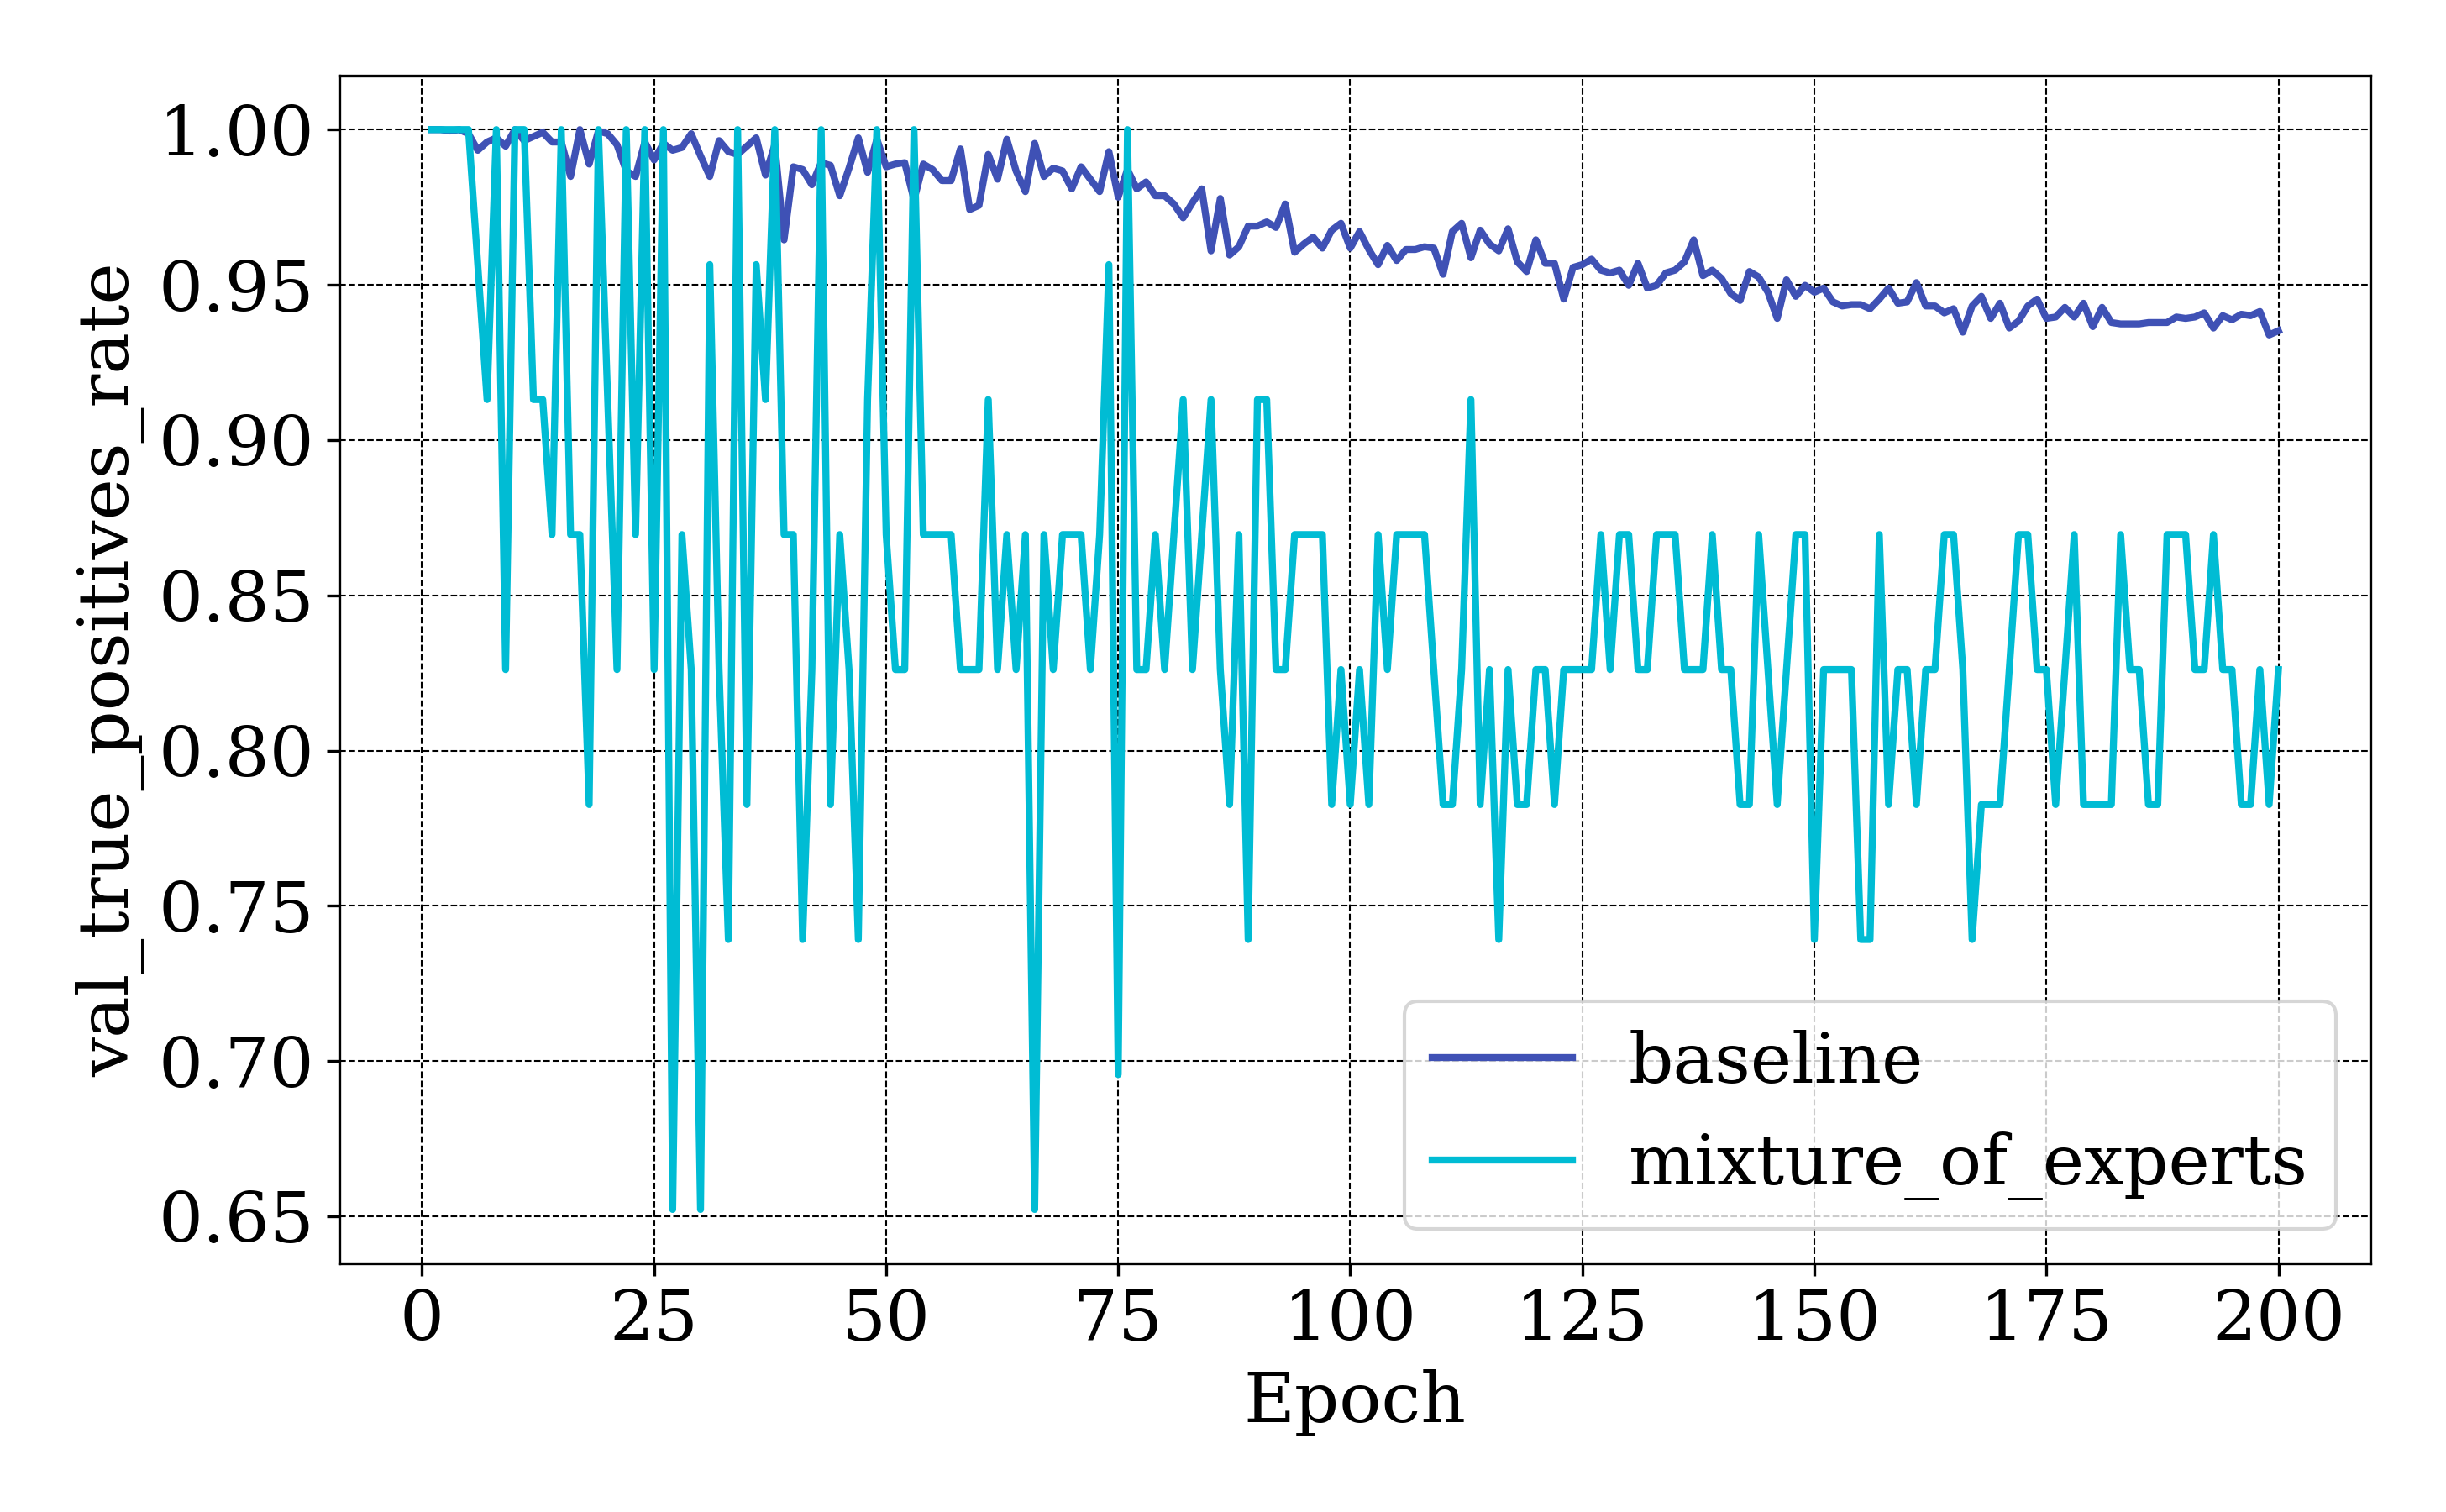
\includegraphics[width=0.45\textwidth]{figures/val_true_positives_rate.png}
        }
    }
    {\caption{Training and validation true positive rates.\label{fig:true_positive_rates}}}
\end{figure}

\end{document}